\documentclass[11pt]{article}
\usepackage[margin=0.95in]{geometry}
\usepackage{amsmath,amssymb}
\usepackage{graphicx}
\usepackage{booktabs,longtable,array}
\usepackage{xcolor}
\usepackage[hidelinks]{hyperref}
\usepackage{enumitem}
\usepackage{caption}
\setlist{itemsep=2pt,topsep=4pt}
\captionsetup{font=small,labelfont=bf}
\setlength{\parskip}{5pt}
\setlength{\parindent}{0pt}
\renewcommand{\arraystretch}{1.15}
\title{Recursion Under Delay: Final Report, Phases 0--3}
\author{}
\date{trm-delay-robust-scaling $\cdot$ final detailed report $\cdot$ 2026-09-22\\[2pt]Covers every phase of the project, from the pilot that motivated it to the last Phase 3 job. Figures are in \texttt{figures/}; analysis files in \texttt{.\allowbreak{}.\allowbreak{}/\allowbreak{}experiments/\allowbreak{}}.}
\begin{document}
\maketitle
\tableofcontents
\clearpage



\section*{Executive summary}\addcontentsline{toc}{section}{Executive summary}



\textbf{The question.} Tiny Recursive Models (TRM) reach state-of-the-art puzzle results with a \textasciitilde{}7M-parameter network by applying one small weight-tied cell many times instead of adding parameters. This project asked whether that trade, iteration in place of parameters, pays off when the network is the actor and critic trunk of a model-free reinforcement-learning agent that controls a plant through delayed actions.



\textbf{The answer, after four phases, 300 training runs and 300 checkpoint evaluations:} it does not, in the regime tested, and the project can now say \emph{why not} with the three confounds that made earlier negatives ambiguous removed.



\begin{itemize}
\item \textbf{The Phase 1 headline replicates and is architectural.} On Pendulum-v1, the one environment every trunk learned, TRM trails a 5.8$\times$ smaller MLP on training return in 12 of 12 seed $\times$ condition pairs (median $-$34.4, p = 0.0005). Matching capacity does not close the gap: TRM loses to a parameter-matched MLP at both 135k ($-$50.2, 0/12) and 788k ($-$27.1, 2/12), while growing the MLP 5.8$\times$ changes nothing ($-$3.8, 5/12).
\item \textbf{Recursion depth is inert.} At fixed parameters, \texttt{H\_cycles} $\in$ \{1, 3, 6\} leaves return unchanged ($-$3.3 and $-$10.9 vs H = 3, 5/12 and 4/12), while cost scales with depth. The shallowest variant trains 2.6$\times$ faster for the same result.
\item \textbf{The value-fit deficit is architectural, not capacity.} TRM's critic loss late in training is 1.45$\times$ and 1.89$\times$ that of a parameter-matched MLP (12/12 pairs each), while the larger MLP fits the value function slightly \emph{better} than the small one. This overturns the capacity reading the Phase 1--2 post-hoc analysis had drawn from the Transformer.
\item \textbf{The deficit is mostly in training, not in the final policy.} Evaluated deterministically, the trunks nearly tie: a residual of 3.6 reward units remains (2/12 pairs), a tenth of the training-return gap. TRM reaches almost the same greedy policy while performing worse throughout training and fitting its value function worse.
\item \textbf{Carrying the latent across steps changes nothing.} Carry-Z, trained with stored-state replay that reproduces the behaviour policy exactly, never beats the latent-resetting TRM in $\geq$5/6 seeds under any delay condition (+4.8, $-$22.0, +16.7).
\item \textbf{Where memory has something to recover, no trunk recovers it.} Hiding the pending-action queue under stochastic delay costs a memoryless MLP 71 reward units (6/6 seeds), so there is headroom for memory. Neither Carry-Z nor a carried LSTM exploits it; the pre-registered interaction has the wrong sign at the decisive condition ($-$40.0, 1/6). A supplementary latent per-episode delay, which memory could in principle identify, gives the same answer: carrying the latent adds nothing (2/6), and the oracle headroom itself is inconsistent (4/6).
\item \textbf{As a controller, TRM is a trade, and a poor one here.} Its greedy policy commands much smoother torque: about 0.4 direction reversals per second against the MLP's 9, in 11/12 pairs, at a return only 3.6 units lower. But it is 65$\times$ slower per decision on one CPU thread (4.1 ms, a 242 Hz ceiling), 11--13$\times$ costlier to train on the same GPU, and less robust to sensor noise, a heavier plant and actuator dropout.
\end{itemize}



\textbf{Status of the hypotheses.} H3, the residual-uncertainty hypothesis that recursion pays only when there is something to infer \emph{and} a carried latent to infer it with, is \textbf{rejected} by its pre-registered gate G2 and by G3. The deflationary capacity account H\_cap is \textbf{also rejected}: capacity changes nothing for either family. What remains is H\_null restricted to this setting: weight-tied recursion, ported without its supervised training discipline, does not transfer to model-free delayed continuous control on the tasks tested. The practical recommendation is unchanged and now firm: use the MLP.



\begin{figure}[htbp]\centering
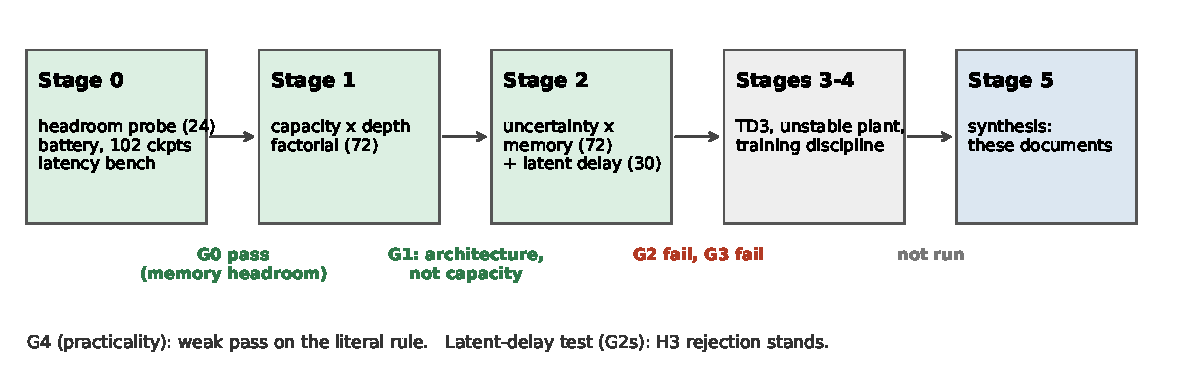
\includegraphics[width=\linewidth,height=0.42\textheight,keepaspectratio]{figures/f1_stage_map.pdf}
\caption{Phase 3 stage map with gate outcomes}
\end{figure}



\medskip



\section*{1. The question and why it was asked}\addcontentsline{toc}{section}{1. The question and why it was asked}



\subsection*{1.1 Tiny Recursive Models and the claim at stake}\addcontentsline{toc}{subsection}{1.1 Tiny Recursive Models and the claim at stake}



TRM (Jolicoeur-Martineau, 2025) replaces depth-by-parameters with depth-by-iteration. A two-layer shared cell recursively refines a latent state conditioned on the input and a candidate answer, then refines the answer, for a fixed number of inner (\texttt{L\_cycles}) and outer (\texttt{H\_cycles}) cycles. With about 7M parameters it reaches 45\% on ARC-AGI-1 and 87\% on Sudoku-Extreme, beating far larger models. The implied claim concerns a \emph{mechanism}, not a task family: iteration with tied weights can substitute for parameter count on problems that reward iterative refinement. If that is true it should matter elsewhere, and embedded or robotic control, where parameters, memory and latency are all scarce, is a natural place to look.



\subsection*{1.2 Why action delay is a fair test}\addcontentsline{toc}{subsection}{1.2 Why action delay is a fair test}



Real controllers sense, compute and actuate with latency. Under a \emph{d}-step action delay, the reward and next observation at time \emph{t} are produced by the action chosen \emph{d} steps earlier, so the raw observation stops being Markov and every stored transition is confounded. The classical fix is observation augmentation: append the queue of committed-but-unapplied actions, which restores a sufficient statistic (Katsikopoulos \& Engelbrecht, 2003). That theorem guarantees only that a sufficient statistic \emph{exists}, not that a small network can \emph{fit} the resulting value function sample-efficiently. Iterative latent refinement, something like a learned state estimator, was a plausible inductive bias for exactly that fitting problem. That was the project's founding bet.



\subsection*{1.3 Scope and boundaries}\addcontentsline{toc}{subsection}{1.3 Scope and boundaries}



The project brief (\texttt{project-config.\allowbreak{}yaml}) fixed four boundaries that held throughout:



\begin{itemize}
\item \textbf{Simulation only.} Embedded deployment, quantisation and hardware budgets were out of scope; Phase 3's latency benchmark is the bridge if that scope reopens.
\item \textbf{Augmentation is the baseline}, not something to re-derive.
\item \textbf{Cost is a first-class metric.} Wall-clock time and parameter count are reported alongside reward on every comparison.
\item \textbf{A rigorous negative result is a valid outcome.} The project was not to bias toward a positive result.
\end{itemize}



The mandatory positioning against prior TRM-for-control work also held. Jain \& Linares (2025) and Wijayatunga \& Armellin (2026) both use TRM \emph{model-based}, refining a control sequence against known dynamics. This project instead tests recursion as an implicit memory or state-estimation mechanism for delay-induced partial observability in \emph{model-free} RL. HRM-Agent (Dang \& Rawlinson, 2025), found during the literature review, is the closest precedent: a recursive reasoning model trained by RL alone that succeeded on discrete mazes, and whose stronger variant carries its latent across timesteps.



\medskip



\section*{2. Phase 0 --- Groundwork (before 2026-09-08)}\addcontentsline{toc}{section}{2. Phase 0 --- Groundwork (before 2026-09-08)}



\subsection*{2.1 The pilot and the augmentation fix}\addcontentsline{toc}{subsection}{2.1 The pilot and the augmentation fix}



The project began from an informal pilot on Pendulum-v1 in this repository. With DDPG, an MLP trunk converged under a 1-step fixed action delay while TRM and Transformer trunks did not. Tracing it (\texttt{augmentation.\allowbreak{}md}) showed the cause was not the trunks. \texttt{DelayedEnv} delayed the action correctly but never told the agent which of its recent actions was about to land, so the replay buffer paired each reward with an action that had no causal role in it. Appending the pending-action queue to the observation fixed it, and the fix was verified exact for fixed delays: all five delay values, ten steps each, zero mismatches against a recorded action sequence. A separate audit of the delay strategies (\texttt{delay-verification.\allowbreak{}md}) found and fixed a bug in \texttt{StochasticDelay}: unclipped samples above \texttt{max\_delay} silently fell back to random actions for the rest of the episode.



With augmentation in place, the pilot reported "comparable reward" for MLP, Transformer and TRM on Pendulum-v1, with TRM costing about 18$\times$ the MLP's training time (55 min vs 3 min per 200 episodes). The project was framed around that observation. Phase 1 later showed the "comparable" part did not survive a controlled replication.



\subsection*{2.2 The TRM port}\addcontentsline{toc}{subsection}{2.2 The TRM port}



The recursive trunk (\texttt{src/\allowbreak{}models/\allowbreak{}trm\_\allowbreak{}control.\allowbreak{}py}, documented in \texttt{notes.md}) ports TRM's mechanism into the same drop-in contract every trunk uses: \texttt{instantiate(model\_\allowbreak{}cfg,\allowbreak{} in\_\allowbreak{}dim=.\allowbreak{}.\allowbreak{}.\allowbreak{})} returns a module whose features feed the actor or critic head. It keeps:



\begin{itemize}
\item the single shared SwiGLU/RMSNorm reasoning cell;
\item the two-latent (\texttt{z\_H}, \texttt{z\_L}) recursion with \texttt{H\_cycles = 3}, \texttt{L\_cycles = 6};
\item fixed initial latent buffers;
\item the one-step gradient truncation, in which all but the final outer cycle run under \texttt{no\_grad}.
\end{itemize}



It drops what has no analogue for a flat continuous observation: token embeddings, self-attention over a length-one sequence, per-puzzle embeddings, and ACT halting with deep supervision. Two properties of the port matter for everything that follows:



\begin{itemize}
\item \textbf{Only 7 of the 21 cell applications per forward pass receive gradient.}
\item \textbf{The latent is re-initialised on every call}, so nothing persists between control steps.
\end{itemize}



The second was later identified as the weaker of HRM-Agent's two variants ("Reset-Z"), and Phase 3 tested the stronger one.



\subsection*{2.3 Scoping, literature review, hypothesis and planning (2026-09-07 to 09-08)}\addcontentsline{toc}{subsection}{2.3 Scoping, literature review, hypothesis and planning (2026-09-07 to 09-08)}



The project was then run as a gated research epic (\texttt{epics/\allowbreak{}trm-delay-robust-scaling/\allowbreak{}}) in autonomous mode.



\begin{itemize}
\item \textbf{Scoping} confirmed that the algorithms (DDPG, TD3, SAC, PPO), the trunks and the augmentation fix already existed and were testable, and that Katana PBS access worked.
\item \textbf{Literature review} (\texttt{docs/\allowbreak{}literature-review/\allowbreak{}review.\allowbreak{}md}) engaged the two mandatory model-based papers and the broader delayed-MDP, POMDP-memory and weight-tied-recursion literature. It stated the model-free versus model-based distinction in a dedicated section.
\item \textbf{Hypothesis ideation} ran three rounds with two reviewers and hit its round cap. Significance stayed at 3 of 5 because the claim rested on one sparse-reward environment and a low-power test. The project escalated, was unblocked by the author ("keep going"), and carried the limitation into the report rather than hiding it. The resulting hypothesis, H1, is stated in \S{}3.
\item \textbf{Experiment planning} added an LSTM trunk (stateless across calls, a mechanistic control), a MountainCarContinuous config, and a first-class results writer. It also replaced a regression design, whose best achievable p at n = 3 was 0.125, with a pooled sign test at n = 6.
\end{itemize}



\medskip



\section*{3. Phase 1 --- Horizon and sparsity (48 runs)}\addcontentsline{toc}{section}{3. Phase 1 --- Horizon and sparsity (48 runs)}



\textbf{Hypothesis H1.} TRM's advantage over the MLP and Transformer is non-decreasing in task complexity. The pre-registered threshold was that the advantage becomes measurable once the horizon is about 5$\times$ Pendulum's and reward is sparse, which MountainCarContinuous-v0 provides (999 steps, one sparse terminal reward).



\textbf{Design.} 4 trunks (MLP, Transformer, TRM, LSTM) $\times$ 2 environments $\times$ 2 delay conditions (none; fixed d = 1 with augmentation) $\times$ 3 seeds = 48 runs, 200 episodes each, CPU only on Katana. The matrix was submitted three times. v1 lost 8 TRM/Transformer MountainCar jobs to walltime, v2 added per-episode logging, and v3 added step-level history and is canonical.



\begin{center}\small\begin{tabular}{>{\raggedright\arraybackslash}p{0.179\linewidth}>{\raggedright\arraybackslash}p{0.276\linewidth}>{\raggedleft\arraybackslash}p{0.124\linewidth}>{\raggedleft\arraybackslash}p{0.300\linewidth}}
\toprule
Comparison & Environment & TRM wins / 6 & one-sided p \\
\midrule
TRM $-$ MLP & Pendulum-v1 & \textbf{0/6} & \textbf{0.016} (a significant \emph{deficit}) \\
TRM $-$ MLP & MountainCarContinuous-v0 & 3/6 & 0.656 \\
TRM $-$ Transformer & Pendulum-v1 & 3/6 & 0.656 \\
TRM $-$ Transformer & MountainCarContinuous-v0 & 4/6 & 0.344 \\
\bottomrule
\end{tabular}\end{center}



\textbf{Findings.}

\begin{enumerate}
\item \textbf{The pilot's parity claim did not survive.} The MLP beat TRM in every seed-pair on Pendulum, by 37.1 reward units under fixed delay ($-$194.0 vs $-$231.1): about 3\% of the span between an untrained policy ($\approx$ $-$1460) and the best run.
\item \textbf{H1's threshold prediction was falsified.} The gap closed on MountainCar in the predicted direction but never approached significance.
\item \textbf{TRM's cost grew with complexity}, from 6.7$\times$ to 12.8$\times$ the MLP's wall-clock.
\item \textbf{The LSTM failed on Pendulum} ($\approx$ $-$1460, an untrained policy) while learning the other tasks, and was flagged as a tuning artefact (Ni et al., 2022).
\end{enumerate}



\begin{figure}[htbp]\centering
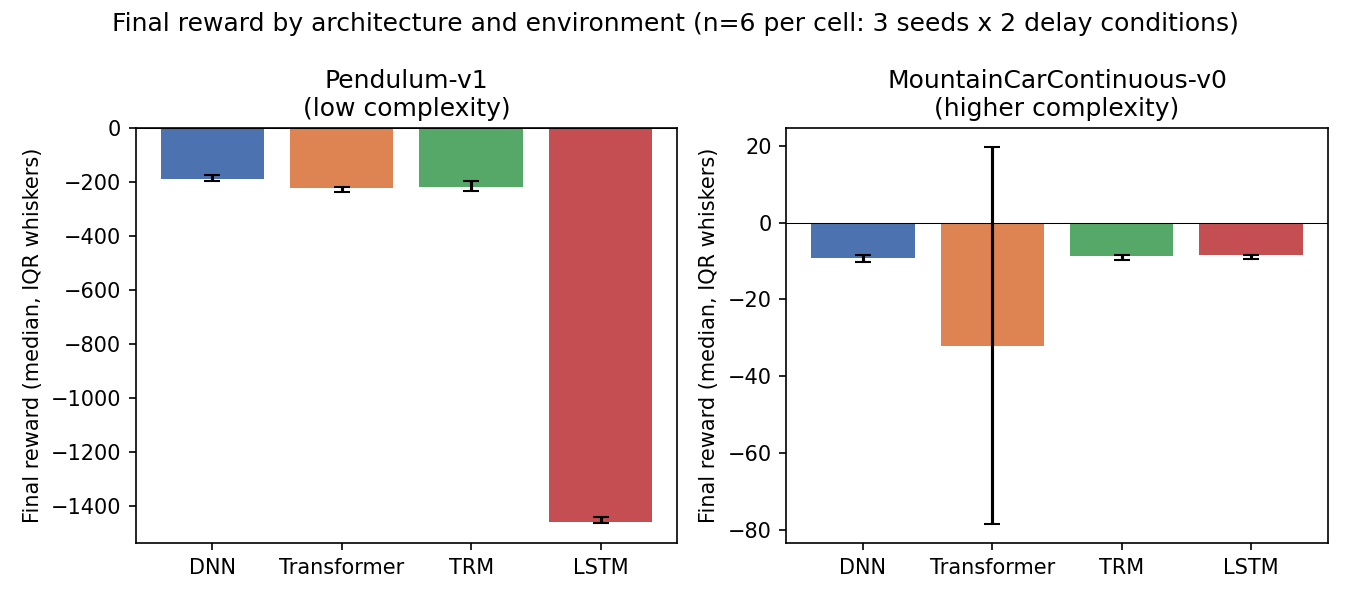
\includegraphics[width=\linewidth,height=0.42\textheight,keepaspectratio]{figures/p12_fig1_reward_by_arch_env.png}
\caption{Phase 1: final reward by trunk and environment}
\end{figure}



\medskip



\section*{4. Phase 2 --- Dimensionality and coupling (54 runs)}\addcontentsline{toc}{section}{4. Phase 2 --- Dimensionality and coupling (54 runs)}



\textbf{Design.} Phase 2 tested a second complexity axis on BipedalWalker-v3 (24-D observation, 4-D action, coupled underactuated dynamics). At the author's request it added two ablations: a \textbf{recursive-structure ablation} (TRM-hier6 with six parallel latent slots, and TRM-singlez with one latent) and an \textbf{augmentation ablation} (fixed delay with the queue removed). The matrix was 6 trunks $\times$ 3 conditions $\times$ 3 seeds = 54 runs, one V100 each. A filename collision silently overwrote three MLP cells. It was caught before analysis, and six jobs were re-run.



\textbf{Findings.}

\begin{enumerate}
\item \textbf{No comparison reached significance in any direction} (TRM $-$ MLP 2/3, TRM $-$ Transformer 0/3, TRM $-$ LSTM 1/3).
\item \textbf{The recursive structure made no detectable difference.} Deltas between base, hier6 and singlez reversed sign from seed to seed, and both variants cost more than the base.
\item \textbf{Augmentation had no clear effect for any trunk.} Two candidates reached the n = 3 ceiling (p = 0.125): TRM-hier6 helped in 3/3 seeds, LSTM hurt in 3/3.
\item \textbf{Cost} was TRM 5.2$\times$, hier6 6.9$\times$ and singlez 8.0$\times$ the MLP's wall-clock on GPU.
\end{enumerate}



\begin{figure}[htbp]\centering
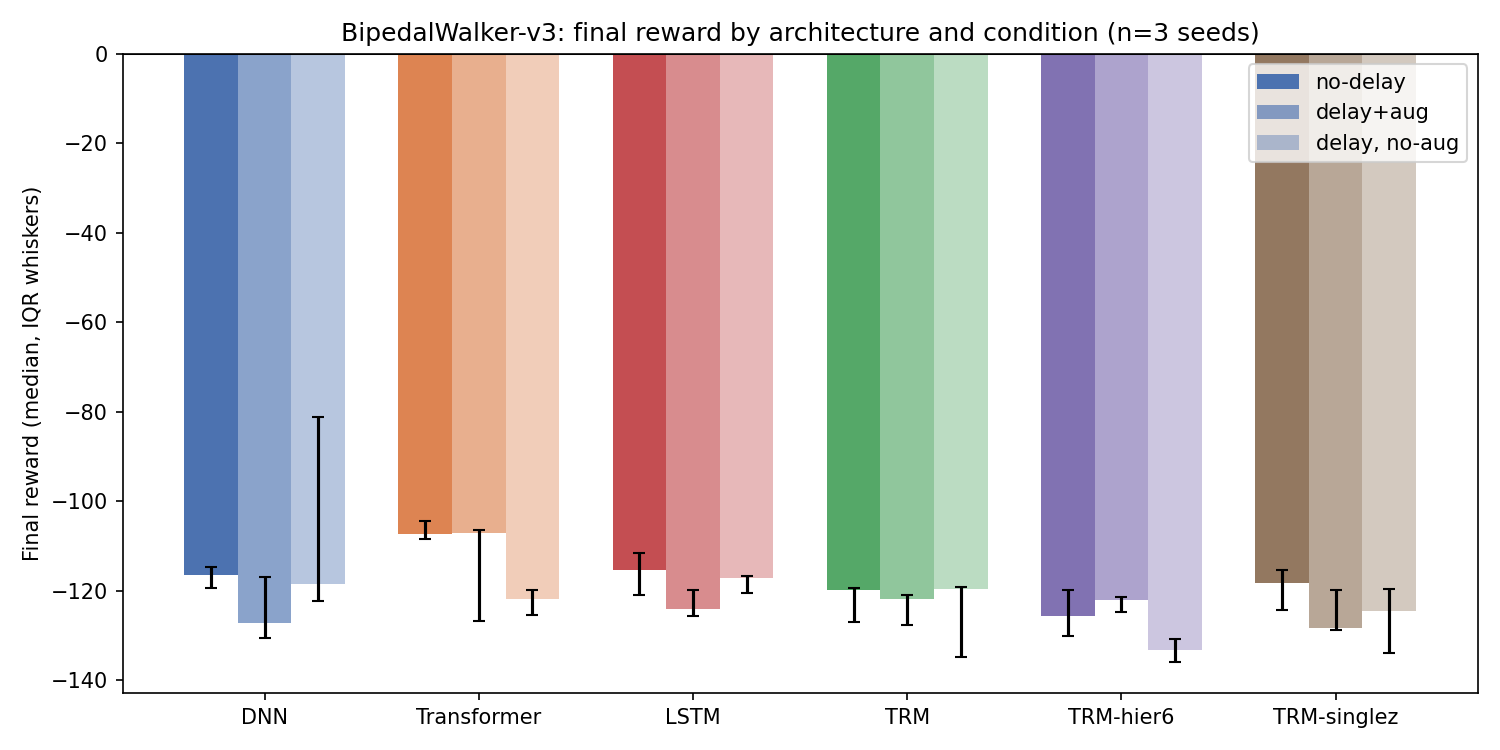
\includegraphics[width=\linewidth,height=0.42\textheight,keepaspectratio]{figures/p12_fig4_reward_by_arch_cond.png}
\caption{Phase 2: final reward by trunk and condition (BipedalWalker-v3)}
\end{figure}



\medskip



\section*{5. Post-hoc analysis of Phases 1--2}\addcontentsline{toc}{section}{5. Post-hoc analysis of Phases 1--2}



Re-analysis of the per-episode telemetry every run had logged, with no new compute, changed what Phases 1--2 meant.



\begin{enumerate}
\item \textbf{Two of three environments are floor effects.} Pendulum-v1 was learned: the best final return was $-$169.9 against a solved threshold of about $-$150. MountainCarContinuous-v0 was exploration-limited and bimodal: median $-$8.9 against a solved threshold of +90, the documented DDPG + OU-noise failure (Matheron et al., 2019). No BipedalWalker-v3 run learned to walk (best $-$81.1 against +300). The complexity-scaling question was therefore never put at risk: it is \emph{untested}, not disconfirmed.
\item \textbf{The recursive trunks fit the value function worse.} TRM's critic loss was higher than the MLP's in 7/7 cells early in training (median 2.72$\times$, p = 0.008), at unchanged learning speed (117 vs 115 episodes to 90\% of span).
\item \textbf{The deficit looked like capacity.} The 797k Transformer showed it too (6/7 early, 7/7 late) and the 167k LSTM did not, so the analysis attributed it to capacity rather than recursion. Phase 3 overturned this attribution (\S{}9.4).
\item \textbf{Three confounds were identified:}
\begin{itemize}
\item \textbf{C-1, capacity:} every recursive trunk held about 788k parameters against the MLP's 135k.
\item \textbf{C-2, latent reset:} the port re-initialises its latent every call, HRM-Agent's weaker variant.
\item \textbf{C-3, nothing to infer:} under fixed d = 1 with augmentation the observation is an exact sufficient statistic.
\end{itemize}
\end{enumerate}



The report was rewritten after author review rejected the first draft. The rejection cited a weak hypothesis, unfair narration, no mechanism, and an unexamined parameter confound. The literature review was then integrated, bringing the report to 26 sources. That integration retracted the novelty claim, because HRM-Agent precedes this work, and identified the latent-reset choice as the most likely single implementation cause.



\begin{figure}[htbp]\centering
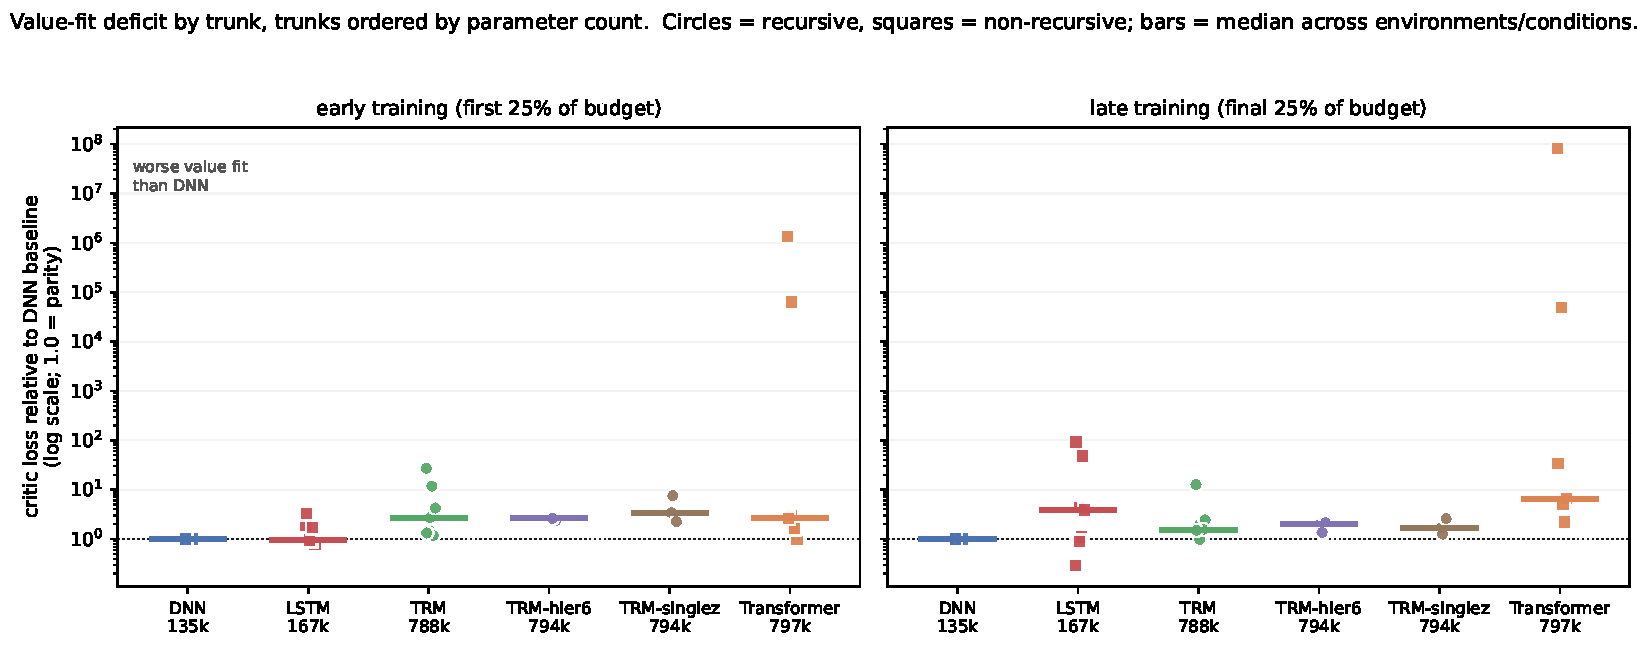
\includegraphics[width=\linewidth,height=0.42\textheight,keepaspectratio]{figures/p12_fig10_capacity_vs_valuefit.pdf}
\caption{Post-hoc: value-fit deficit by trunk ordered by parameter count (Phases 1--2)}
\end{figure}



\medskip



\section*{6. Phase 3 design}\addcontentsline{toc}{section}{6. Phase 3 design}



\subsection*{6.1 Hypothesis and alternatives}\addcontentsline{toc}{subsection}{6.1 Hypothesis and alternatives}



\begin{quote}\textbf{H3 --- residual-uncertainty hypothesis.} Weight-tied recursion earns its cost in model-free continuous control only where \textbf{(i)} the agent's conditioning leaves residual state uncertainty that iteration could resolve, \textbf{and (ii)} the trunk carries information across decision steps so iteration has something to accumulate. Phases 1--2 satisfied neither.\end{quote}



H3 was tested against two deflationary accounts: \textbf{H\_cap} (the deficits track parameter count; recursion is irrelevant) and \textbf{H\_null} (recursive refinement does not transfer to model-free continuous control under any conditioning). Its load-bearing prediction (H3.2) was an \emph{interaction}: Carry-Z $-$ MLP $\leq$ 0 under fixed, known delay but > 0 where there is something to infer. A capacity story cannot flip that sign using identical networks.



\subsection*{6.2 Stages and gates}\addcontentsline{toc}{subsection}{6.2 Stages and gates}



The plan (\texttt{papers/\allowbreak{}phase3/\allowbreak{}plan.\allowbreak{}md}, 2026-09-14) laid out six gated stages, each with a decision rule written before its compute:



\begin{center}\small\begin{tabular}{>{\raggedright\arraybackslash}p{0.063\linewidth}>{\raggedright\arraybackslash}p{0.581\linewidth}>{\raggedright\arraybackslash}p{0.262\linewidth}}
\toprule
Stage & Question & Gate \\
\midrule
0 & Is there headroom for inference? What do the banked checkpoints already say about control quality? & G0 headroom; G4 practicality \\
1 & Capacity or recursion? 2$\times$2 of \{MLP, TRM\} $\times$ \{135k, 788k\}, plus \texttt{H\_cycles} $\in$ \{1, 6\} & G1 attribution, no kill branch \\
2 & Uncertainty $\times$ memory: \{MLP, Reset-Z, Carry-Z, carried LSTM\} $\times$ \{C1, C3, C4\} & G2 interaction; failure rejects H3 \\
3 & Does it generalise? TD3 cross-check; InvertedDoublePendulum-v5 & G3 continuity \\
4 & Restore the training discipline: no truncation, per-cycle supervision, DEQ & --- \\
5 & Synthesis & always \\
\bottomrule
\end{tabular}\end{center}



The delay conditions were:

\begin{itemize}
\item \textbf{C1:} fixed d = 1 with the queue (the Phase 1 condition).
\item \textbf{C3:} d \textasciitilde{} U\{0..4\} resampled every step, with the 4-slot queue.
\item \textbf{C4:} the same delay with the queue withheld.
\end{itemize}



\subsection*{6.3 The 2026-09-17 plan review}\addcontentsline{toc}{subsection}{6.3 The 2026-09-17 plan review}



A review written three days after the plan (\texttt{papers/\allowbreak{}summary.\allowbreak{}md} \S{}7) found the plan's diagnosis and gating sound. Its one critical objection was that \textbf{C3 contains no inferable hidden state in this codebase.} With the delay drawn fresh each step, every action that can reach the plant is already in the augmented observation, so an MLP sees everything a perfect memory would. Its recommendations, and what Phase 3 did with each:



\begin{center}\small\begin{tabular}{>{\raggedright\arraybackslash}p{0.522\linewidth}>{\raggedright\arraybackslash}p{0.412\linewidth}}
\toprule
Review recommendation & Adopted? \\
\midrule
Replace the uncertainty axis with a \textbf{per-episode latent delay} (d drawn once per episode) that memory can identify & \textbf{Yes, as a supplementary test} after G2 (\S{}9.6); the primary Stage 2 ran C3/C4 as planned \\
Add a fixed d = 4 control to separate delay size from uncertainty & No (moot once G2 found no interaction to explain) \\
Make Carry-Z $-$ carried LSTM and Carry-Z $-$ Reset-Z co-primary & Both computed and reported (\S{}9.5); Carry-Z $-$ Reset-Z is G3 \\
Tighten gates (10 seeds for MLP arms; p $\leq$ 0.05) & No: 6 seeds and $\geq$5/6 throughout, as pre-registered \\
Pre-register how off-nominal delays are shown to fixed-width policies & \textbf{Yes} (A-5 battery design: the trained queue width is kept) \\
Engineer the carried LSTM's off-policy machinery & \textbf{Yes} (same stored-state replay as Carry-Z); not tuned \\
Correct the U\{0..4\} description & \textbf{Yes} (amendment A-4) \\
\bottomrule
\end{tabular}\end{center}



This review was not consulted before execution began on 2026-09-21. Execution reached its central point independently (amendment A-1 below) but not its recommended fix. The latent-delay test was therefore added afterwards, with its rule written before its data. It is labelled supplementary throughout.



\subsection*{6.4 Amendments recorded before submission (2026-09-21)}\addcontentsline{toc}{subsection}{6.4 Amendments recorded before submission (2026-09-21)}



\begin{itemize}
\item \textbf{A-1, theory check.} Under i.i.d. per-step delay with a fully observed plant and the 4-slot queue, the augmented observation is already Markov, so the oracle arm (realised past delay) is predicted null and G0 as written would fail by construction.
\item \textbf{A-2, extra arm and amended G0.} Arm A4 (stochastic delay, no queue) was added, and G0 passes on either oracle headroom (A3 $-$ A2) or memory headroom (A2 $-$ A4).
\item \textbf{A-3, co-primary condition.} C4 became co-primary with C3 for G2.
\item \textbf{A-4, exact delay distribution.} U\{0..4\} is now drawn exactly; the old \texttt{uniform} option under-weights the endpoints.
\item \textbf{A-5, compute placement.} Every job ran on a GPU node, the battery ran as 12 shard jobs, latency as one job, and every result records its device.
\item \textbf{A-6, Stage 2 inputs.} Every Stage 2 trunk, the MLP included, also sees its previous action (Ni et al., 2022), so the trunks differ only in architecture and memory. \S{}9.5 shows this choice had a side effect.
\end{itemize}



\medskip



\section*{7. Phase 3 engineering and verification}\addcontentsline{toc}{section}{7. Phase 3 engineering and verification}



Every new component was verified before it was used for a result.



\begin{center}\small\begin{tabular}{>{\raggedright\arraybackslash}p{0.184\linewidth}>{\raggedright\arraybackslash}p{0.355\linewidth}>{\raggedright\arraybackslash}p{0.367\linewidth}}
\toprule
Component & What it does & Verification \\
\midrule
\texttt{DelayedEnv} extensions (\texttt{src/delays.py}) & exact \texttt{uniform\_int} delay, delay oracle, configurable queue width, previous-action wrapper, per-episode latent delay & bit-identical to the old wrapper on all existing delay $\times$ augmentation configurations (20 before the latent delay, re-checked after) \\
\texttt{src/\allowbreak{}perturb.\allowbreak{}py} & sensor noise, actuator dropout, pendulum mass/length scaling, all below the delay wrapper & exercised by 300 battery evaluations \\
\texttt{src/eval.py}, \texttt{w0\_eval.py} & rebuilds any checkpoint from its results file; deterministic batched rollouts under 20 grid points; control-quality metrics & rebuilt parameter count equals the recorded one for all 300 checkpoints evaluated \\
\texttt{TRMCarryTrunk}, \texttt{LSTMCarryTrunk} & latent / hidden state carried across steps; \texttt{forward(x,\allowbreak{} carry) -> (features,\allowbreak{} carry)} & Carry-Z parameters identical to Reset-Z's in every condition \\
Stored-state replay (DDPG and TD3) & actor and critic carries stored before and after every step; updates start each trunk from the carry it acted from & feeding stored carries back reproduces the behaviour policy's actions and next carries with \textbf{zero error} \\
Stateless paths after the changes & --- & DDPG and TD3 updates, weights and actions identical to the old code at agent level \\
Seeding & warmup \texttt{action\_\allowbreak{}space.\allowbreak{}sample()} was unseeded in Phases 1--2; now seeded from the run seed & runs reproducible end to end; every arm's first episode now identical \\
\texttt{bench\_\allowbreak{}latency.\allowbreak{}py} & batch-1 and batch-256 decision latency, CPU (1 thread) and GPU, plus full update cost & one job on a Xeon Gold 6342 + A100 \\
Job manager \texttt{p3.py} & per-stage frozen code snapshots, ledger, live status JSON & two GPU smoke jobs passed before any stage was submitted \\
\bottomrule
\end{tabular}\end{center}



A live run board (\texttt{https:/\allowbreak{}/\allowbreak{}claude.\allowbreak{}ai/\allowbreak{}artifact/\allowbreak{}8BBqkDsAm2ocizL1kTn6nB}) was polled about every 19 minutes during execution.



\medskip



\section*{8. Phase 3 execution log}\addcontentsline{toc}{section}{8. Phase 3 execution log}



\begin{center}\small\begin{tabular}{>{\raggedright\arraybackslash}p{0.364\linewidth}>{\raggedleft\arraybackslash}p{0.053\linewidth}>{\raggedright\arraybackslash}p{0.489\linewidth}}
\toprule
Stage & Jobs & Notes \\
\midrule
Smoke tests & 2 & A100; all arms, battery and latency passed \\
S0.1 headroom probe & 24 & MLP runs about 3 min each on GPU \\
S0.2 battery (102 banked checkpoints) & 12 & 0 parameter-rebuild mismatches \\
S0.2 latency benchmark & 1 & Xeon Gold 6342 (1 thread) + A100 \\
Stage 1 & 72 & 5 crashed on an unsupported GPU and were resubmitted \\
Stage 2 & 72 & from a frozen snapshot, MLP = \texttt{dnn} per G1 \\
Supplementary latent-delay test & 30 & rule fixed before submission \\
Battery over Stage 0.1, 1 and 2 checkpoints & 12 & 168 checkpoints \\
Battery top-up & 1 & 6 checkpoints skipped by a filename collision (incident 3) \\
Battery, latent-delay checkpoints & 5 & 30 checkpoints \\
\textbf{Total} & \textbf{231} & plus 5 resubmissions; 0 unrecovered failures \\
\bottomrule
\end{tabular}\end{center}



Four incidents are worth recording.

\begin{enumerate}
\item \textbf{Unsupported GPU (k207).} Five Stage 1 MLP jobs landed on an RTX PRO 6000 Blackwell node (sm\_120), for which the venv's torch 2.5.1 + cu121 build has no kernels. All queued jobs were altered to request \texttt{gpu\_\allowbreak{}rp6000=False}, which excludes only that node, and the five were resubmitted.
\item \textbf{Queue routing.} Jobs requesting 4--6 h queued in \texttt{mechgpu12}, which reaches only group-owned nodes, and only two ran at a time. Jobs of $\leq$ 2 h route to \texttt{mechgpu2}, which reaches every GPU node. Because a site hook forbids changing a queued job's walltime, the 46 queued TRM jobs were deleted and resubmitted at 1:59 from the same frozen snapshot. The first attempt at this failed its resubmits because \texttt{qstat} truncated job names; all 46 were then resubmitted from the ledger's full names.
\item \textbf{Battery filename collision.} Stage 0's arm A1 and Stage 1's \texttt{dnn} at fixed delay produce identical results basenames. The battery therefore skipped the six Stage 1 checkpoints as "already done". They were identified by \texttt{model\_id}, evaluated in a separate top-up job, and every battery row is attributed to its stage by \texttt{model\_id}, never by filename.
\item \textbf{Hardware heterogeneity.} Runs landed on V100, A100, L40S and H100 GPUs. Every result records its device, and the cost ledger compares trunks within a GPU model.
\end{enumerate}



\medskip



\section*{9. Phase 3 results}\addcontentsline{toc}{section}{9. Phase 3 results}



All returns are the final 100-episode average of \emph{training} return (the pre-registered metric, as in Phases 1--2) unless marked as deterministic evaluation. "k/n" means k of n paired differences are positive; p is a sign test.



\subsection*{9.1 Stage 0.1 --- Headroom (G0)}\addcontentsline{toc}{subsection}{9.1 Stage 0.1 --- Headroom (G0)}



Four MLP arms on Pendulum-v1, 6 seeds each:



\begin{center}\small\begin{tabular}{llr}
\toprule
Arm & Condition & Median final return \\
\midrule
A1 & fixed d = 1 + queue & $-$176.6 \\
A2 & stochastic U\{0..4\} + queue & $-$234.0 \\
A3 & A2 + realised delay exposed (the oracle) & $-$289.3 \\
A4 & stochastic U\{0..4\}, no queue & $-$306.6 \\
\bottomrule
\end{tabular}\end{center}



\begin{center}\small\begin{tabular}{>{\raggedright\arraybackslash}p{0.348\linewidth}>{\raggedleft\arraybackslash}p{0.098\linewidth}>{\raggedleft\arraybackslash}p{0.082\linewidth}>{\raggedleft\arraybackslash}p{0.092\linewidth}>{\raggedleft\arraybackslash}p{0.121\linewidth}>{\raggedright\arraybackslash}p{0.081\linewidth}}
\toprule
Contrast & Median diff & Pooled SD & Positive & p (one-sided) & Passes? \\
\midrule
Oracle headroom A3 $-$ A2 (pre-registered) & $-$39.6 & 96.9 & 0/6 & 1.000 & no \\
Memory headroom A2 $-$ A4 (amendment A-2) & +70.8 & 49.5 & 6/6 & 0.016 & \textbf{yes} \\
Cost of stochastic delay A1 $-$ A2 & +53.3 & 19.2 & 6/6 & 0.016 & --- \\
\bottomrule
\end{tabular}\end{center}



\textbf{G0 passes, on the amended rule only.} Showing the realised delay made the MLP \emph{worse} in all six seeds, as A-1 predicted: the input carries no usable information and costs something to ignore. Hiding the queue costs 71 reward units, so there \emph{is} headroom for a trunk that can rebuild the queue from its own history. That made C4 the decisive Stage 2 condition.



\begin{figure}[htbp]\centering
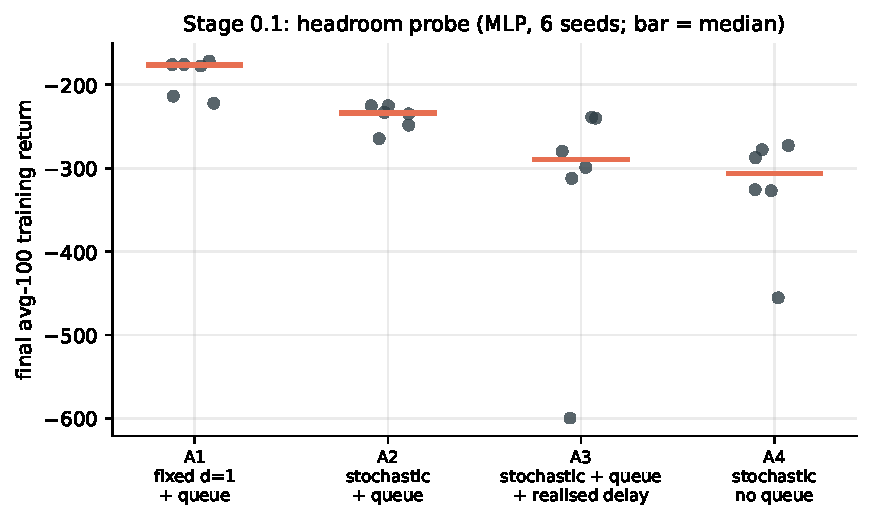
\includegraphics[width=\linewidth,height=0.42\textheight,keepaspectratio]{figures/f2_headroom.pdf}
\caption{Stage 0.1 headroom probe}
\end{figure}



\subsection*{9.2 Stage 0.2 --- The banked checkpoints as controllers (G4)}\addcontentsline{toc}{subsection}{9.2 Stage 0.2 --- The banked checkpoints as controllers (G4)}



All 102 Phase 1--2 checkpoints were re-evaluated with no retraining: 20 deterministic episodes on unseen seeds, plus 10-episode grids for delay mismatch (d = 0\ldots{}5, keeping the trained queue width), sensor noise ($\sigma$ = 0.01--0.10 of the observation half-range), pendulum mass and length (0.7--1.3$\times$) and actuator dropout (5\%, 10\%). The interpretable cells are Pendulum-v1 (n = 3 seeds each):



\begin{center}\small\begin{tabular}{>{\raggedright\arraybackslash}p{0.186\linewidth}>{\raggedleft\arraybackslash}p{0.171\linewidth}>{\raggedleft\arraybackslash}p{0.137\linewidth}>{\raggedleft\arraybackslash}p{0.103\linewidth}>{\raggedleft\arraybackslash}p{0.144\linewidth}>{\raggedleft\arraybackslash}p{0.081\linewidth}}
\toprule
Trunk (fixed d = 1 + queue) & Nominal IQM [95\% CI] & Command rate abs($\Delta$u) & Reversals / s & Sensor noise $\sigma$ = 0.05 & Delay d = 3 \\
\midrule
MLP 135k & $-$119.9 [$-$122.6, $-$96.3] & 0.729 & 3.9 & $-$145.2 & $-$406.8 \\
TRM 788k & $-$124.2 [$-$133.4, $-$99.3] & 0.642 & 0.8 & $-$337.9 & $-$379.8 \\
Transformer 797k & $-$122.0 [$-$160.6, $-$96.5] & 1.299 & 7.7 & $-$260.3 & $-$509.2 \\
LSTM 167k & $-$1146.2 [$-$1526.5, $-$188.1] & 0.000 & 0.0 & $-$1477.6 & $-$1489.7 \\
\bottomrule
\end{tabular}\end{center}



\begin{itemize}
\item \textbf{Every trunk that learned reaches the same greedy policy quality} (IQM about $-$120).
\item \textbf{At n = 3 the Phase 1--2 smoothness signal is inside seed noise.} That signal came from exploration-noisy actions. Deterministically, command rate varies more across seeds of one trunk than between trunks (MLP 0.10--0.78, TRM 0.13--0.79). \S{}9.7 revisits this at n = 12 and finds a real difference in direction reversals.
\item \textbf{All learned trunks share one delay envelope:} fine at d $\leq$ 2, collapsing at d $\geq$ 3.
\item \textbf{TRM degrades faster under sensor noise} than the MLP.
\end{itemize}



\textbf{G4 passes weakly, on the literal rule.} TRM is non-dominated against the MLP on command rate at a tied return and admits 100 Hz control, but the margin is inside seed noise. The LSTM also satisfies the rule, but degenerately: a policy that never learned is maximally smooth. The rule did not exclude that case and is reported as written.



\subsection*{9.3 Latency --- can it close a real control loop?}\addcontentsline{toc}{subsection}{9.3 Latency --- can it close a real control loop?}



Actor forward pass per decision, batch 1, including host transfers:



\begin{center}\small\begin{tabular}{>{\raggedright\arraybackslash}p{0.189\linewidth}>{\raggedleft\arraybackslash}p{0.189\linewidth}>{\raggedleft\arraybackslash}p{0.094\linewidth}>{\raggedleft\arraybackslash}p{0.094\linewidth}>{\raggedleft\arraybackslash}p{0.283\linewidth}}
\toprule
Trunk & 1 CPU thread p99 & Max rate & A100 p99 & Update (batch 128), A100 \\
\midrule
MLP 135k & 0.064 ms & 15.5 kHz & 0.18 ms & 3.7 ms \\
MLP 788k & 0.119 ms & 8.4 kHz & 0.18 ms & 3.7 ms \\
LSTM (carried) & 0.129 ms & 7.7 kHz & 0.26 ms & 4.9 ms \\
Transformer & 0.512 ms & 2.0 kHz & 0.61 ms & 14.2 ms \\
TRM H = 1 & 1.42 ms & 703 Hz & 1.86 ms & 24.2 ms \\
TRM 136k & 2.69 ms & 371 Hz & 5.25 ms & 40.8 ms \\
TRM 788k (H = 3) & 4.13 ms & 242 Hz & 5.31 ms & 41.3 ms \\
TRM Carry-Z & 4.11 ms & 243 Hz & 5.35 ms & 41.8 ms \\
TRM H = 6 & 7.59 ms & 132 Hz & 10.0 ms & 66.3 ms \\
\bottomrule
\end{tabular}\end{center}



\begin{itemize}
\item \textbf{TRM supports a 100 Hz loop but not 500 Hz or 1 kHz.} It is 65$\times$ the MLP's latency, and a GPU makes batch-1 decisions \emph{slower} because the 21 sequential cell applications are bound by kernel-launch overhead.
\item \textbf{Latency scales with depth, not width.} TRM 136k is barely faster than TRM 788k, while H = 1 is about 3$\times$ faster than H = 3.
\end{itemize}



\begin{figure}[htbp]\centering
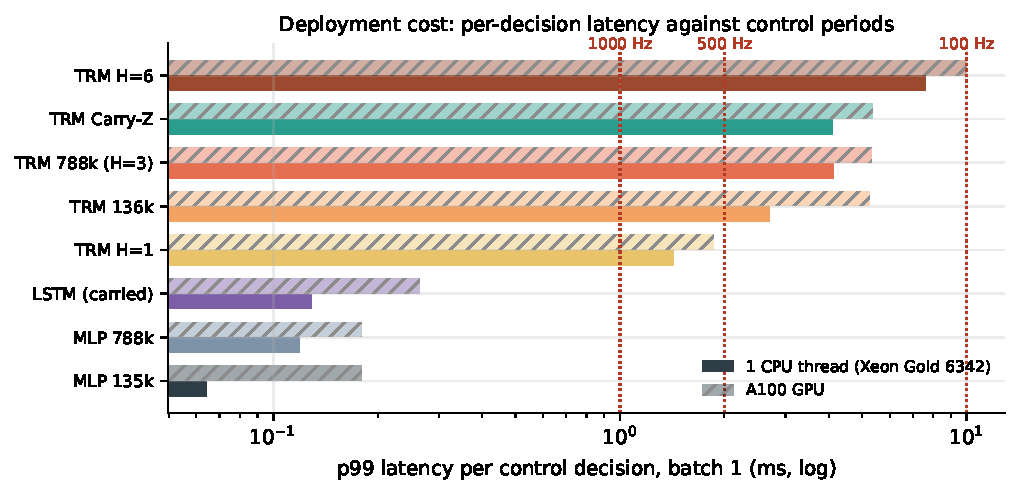
\includegraphics[width=\linewidth,height=0.42\textheight,keepaspectratio]{figures/f6_latency.pdf}
\caption{Per-decision latency against control periods}
\end{figure}



\subsection*{9.4 Stage 1 --- Capacity or recursion? (G1)}\addcontentsline{toc}{subsection}{9.4 Stage 1 --- Capacity or recursion? (G1)}



Six arms $\times$ \{no delay, fixed d = 1 + queue\} $\times$ 6 seeds (n = 12 pairs per contrast):



\begin{center}\small\begin{tabular}{>{\raggedright\arraybackslash}p{0.158\linewidth}>{\raggedleft\arraybackslash}p{0.081\linewidth}>{\raggedleft\arraybackslash}p{0.102\linewidth}>{\raggedleft\arraybackslash}p{0.213\linewidth}>{\raggedleft\arraybackslash}p{0.136\linewidth}>{\raggedleft\arraybackslash}p{0.132\linewidth}}
\toprule
Arm & Params & Median return & Deterministic eval (last 5) & Median wall-clock & Critic loss, late \\
\midrule
MLP 135k (\texttt{dnn}) & 134,914 & $-$174.5 & $-$161.0 & 3.0 min & 11.0 \\
TRM 136k (\texttt{trm\_small}) & 135,654 & $-$232.4 & $-$169.9 & 31.7 min & 16.8 \\
MLP 788k (\texttt{dnn\_large}) & 788,114 & $-$177.3 & $-$164.0 & 3.0 min & 9.2 \\
TRM 788k (\texttt{trm}) & 787,842 & $-$207.9 & $-$162.3 & 32.2 min & 17.4 \\
TRM H = 1 & 787,842 & $-$198.9 & $-$165.1 & 12.4 min & 14.4 \\
TRM H = 6 & 787,842 & $-$218.4 & $-$163.8 & 35.2 min & 18.7 \\
\bottomrule
\end{tabular}\end{center}



\begin{center}\small\begin{tabular}{>{\raggedright\arraybackslash}p{0.354\linewidth}>{\raggedleft\arraybackslash}p{0.130\linewidth}>{\raggedleft\arraybackslash}p{0.092\linewidth}>{\raggedleft\arraybackslash}p{0.115\linewidth}>{\raggedleft\arraybackslash}p{0.159\linewidth}}
\toprule
Contrast (n = 12) & Training return & Positive & p (two-sided) & Deterministic eval \\
\midrule
TRM 136k $-$ MLP 135k & $-$50.2 & 0/12 & 0.0005 & $-$4.4 (5/12) \\
TRM 788k $-$ MLP 788k & $-$27.1 & 2/12 & 0.039 & +0.3 (6/12) \\
MLP 788k $-$ MLP 135k & $-$3.8 & 5/12 & 0.77 & $-$2.2 (4/12) \\
TRM 788k $-$ TRM 136k & +20.7 & 7/12 & 0.77 & +2.7 (8/12) \\
TRM H = 1 $-$ H = 3 & $-$3.3 & 5/12 & 0.77 & $-$2.8 (5/12) \\
TRM H = 6 $-$ H = 3 & $-$10.9 & 4/12 & 0.39 & $-$2.2 (4/12) \\
TRM 788k $-$ MLP 135k (the Phase 1 headline) & $-$34.4 & 0/12 & 0.0005 & $-$2.5 (2/12) \\
\bottomrule
\end{tabular}\end{center}



\textbf{G1: the deficit is architecture-family, not capacity.} TRM loses at both matched sizes, and capacity moves neither family. Per the pre-registered rule, Stage 2's MLP is \texttt{dnn}. Four further findings sharpen this.



\begin{enumerate}
\item \textbf{Reproduction.} On new code, new hardware and seeded warmup, the Phase 1 headline reproduces: TRM $-$ MLP $-$34.4 at n = 12 (0/12), against Phase 1's $-$32.8 at n = 6 (0/6). The MLP medians also match Phase 1 (no delay $-$174.3 vs $-$174.0).
\item \textbf{Depth is inert.} H = 1 has 7 cell applications per pass against H = 3's 21, and H = 6 has 42, yet returns do not move. Only 7 applications receive gradient at any depth. This reproduces Roye-Azar et al.'s "shallow effective recursion" outside its original domain.
\item \textbf{The value-fit deficit is architectural.} Late critic loss is 1.45$\times$ (TRM 136k vs MLP 135k) and 1.89$\times$ (TRM 788k vs MLP 788k), 12/12 pairs each, while the 788k MLP fits value slightly \emph{better} than the 135k one (0.87$\times$, 3/12). Removing the outer recursion reduces but does not remove the deficit (H = 1 vs MLP: 1.34$\times$, 10/12). This reverses the Phase 1--2 post-hoc attribution to capacity, which rested on the Transformer. That Transformer deficit is now better read as the Transformer's own.
\item \textbf{The deficit lives mostly in training, not in the final policy.} On deterministic evaluation episodes, which share initial states across arms within a seed, the gaps shrink to a few reward units. The battery (\S{}9.7), on unseen seeds, puts the residual at 3.6 units (2/12, p = 0.039): small but consistent. TRM nearly reaches the MLP's greedy policy, but fits its critic worse and performs worse under exploration noise throughout training.
\end{enumerate}



\begin{figure}[htbp]\centering
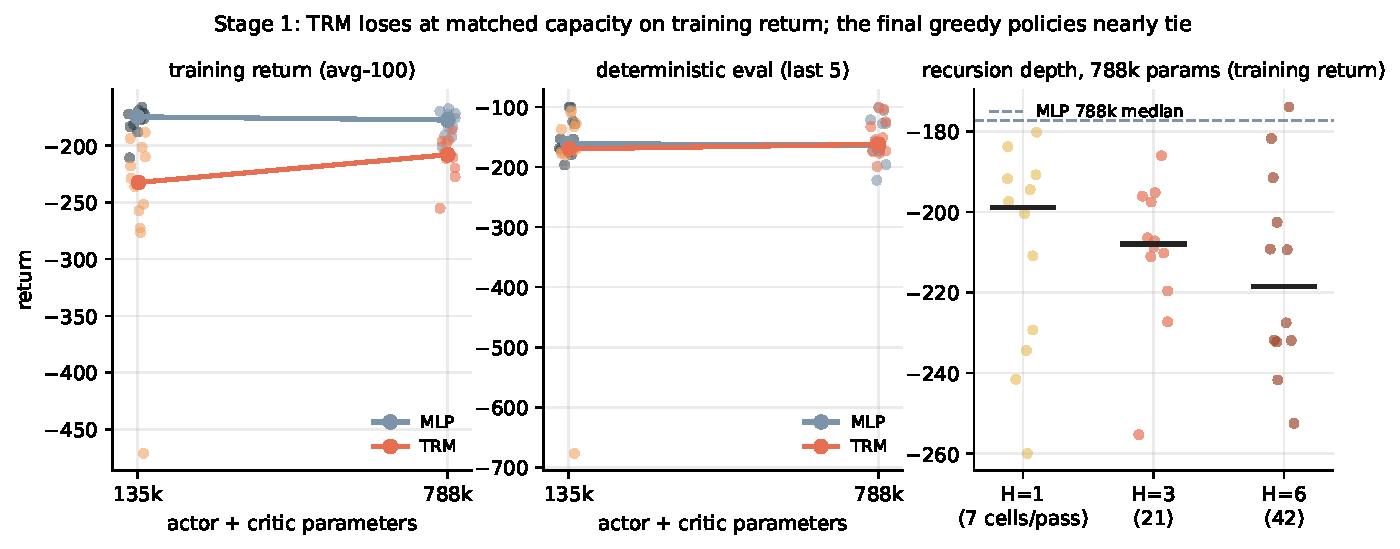
\includegraphics[width=\linewidth,height=0.42\textheight,keepaspectratio]{figures/f3_capacity_depth.pdf}
\caption{Stage 1: capacity $\times$ depth}
\end{figure}



\begin{figure}[htbp]\centering
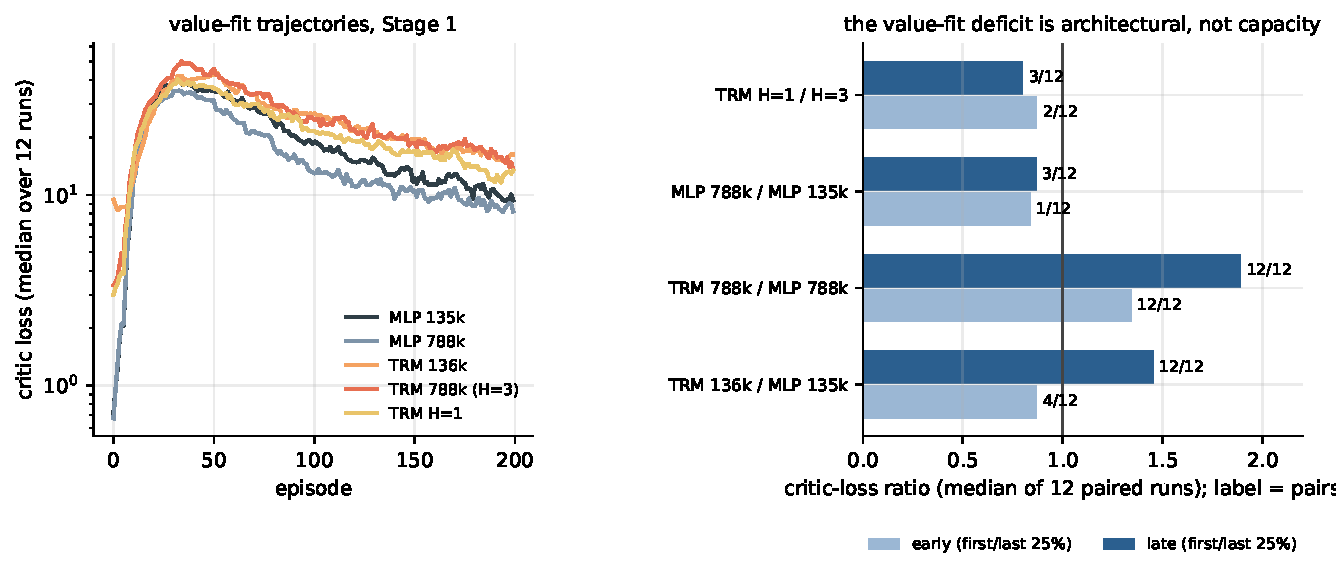
\includegraphics[width=\linewidth,height=0.42\textheight,keepaspectratio]{figures/f4_value_fit.pdf}
\caption{Value fit at matched capacity}
\end{figure}



\begin{figure}[htbp]\centering
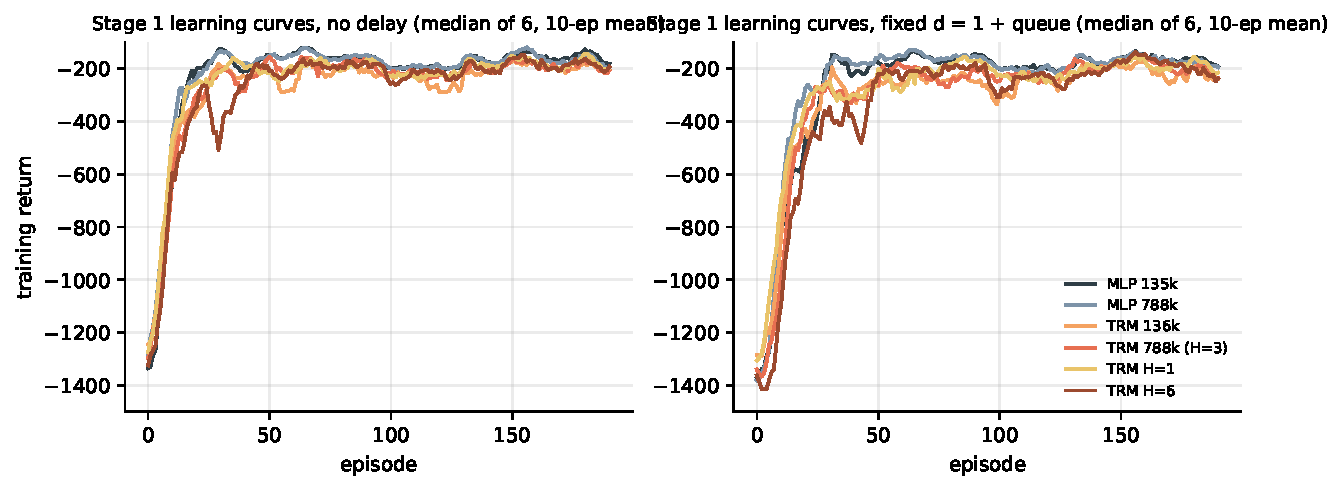
\includegraphics[width=\linewidth,height=0.42\textheight,keepaspectratio]{figures/f10_learning_curves.pdf}
\caption{Stage 1 learning curves}
\end{figure}



\subsection*{9.5 Stage 2 --- Uncertainty $\times$ memory (G2, G3)}\addcontentsline{toc}{subsection}{9.5 Stage 2 --- Uncertainty $\times$ memory (G2, G3)}



Four trunks $\times$ three conditions $\times$ 6 seeds. Every trunk also sees its previous action (A-6).



\begin{center}\small\begin{tabular}{>{\raggedright\arraybackslash}p{0.166\linewidth}>{\raggedleft\arraybackslash}p{0.190\linewidth}>{\raggedleft\arraybackslash}p{0.249\linewidth}>{\raggedleft\arraybackslash}p{0.273\linewidth}}
\toprule
Trunk & C1 fixed + queue & C3 stochastic + queue & C4 stochastic, no queue \\
\midrule
MLP 135k & $-$178.3 & $-$293.7 & $-$235.4 \\
TRM Reset-Z & $-$226.8 & $-$270.5 & $-$333.9 \\
TRM Carry-Z & $-$214.5 & $-$300.1 & $-$333.1 \\
LSTM (carried) & $-$252.1 & $-$786.3 & $-$370.9 \\
\bottomrule
\end{tabular}\end{center}



\begin{center}\small\begin{tabular}{>{\raggedright\arraybackslash}p{0.389\linewidth}>{\raggedleft\arraybackslash}p{0.229\linewidth}>{\raggedleft\arraybackslash}p{0.130\linewidth}>{\raggedleft\arraybackslash}p{0.130\linewidth}}
\toprule
Contrast (n = 6) & Median & Positive & p (two-sided) \\
\midrule
\textbf{G2} interaction [Carry-Z $-$ MLP], C3 $-$ C1 & +20.4 & 3/6 & 1.00 \\
\textbf{G2} interaction [Carry-Z $-$ MLP], C4 $-$ C1 & $-$40.0 & 1/6 & 0.22 \\
\textbf{G3} Carry-Z $-$ Reset-Z at C1 / C3 / C4 & +4.8 / $-$22.0 / +16.7 & 4/6, 3/6, 3/6 & $\geq$ 0.69 \\
Carry-Z $-$ MLP at C1 / C3 / C4 & $-$29.5 / $-$18.2 / $-$81.5 & 1/6, 2/6, 1/6 & --- \\
Carry-Z $-$ LSTM at C1 / C3 / C4 & +56.5 / +500.0 / +45.0 & 6/6, 6/6, 5/6 & --- \\
Carried LSTM $-$ MLP at C1 / C3 / C4 & $-$66.4 / $-$381.6 / $-$137.2 & 0/6, 1/6, 1/6 & --- \\
\bottomrule
\end{tabular}\end{center}



\textbf{G2 fails and H3 is rejected.} The interaction does not appear at either co-primary condition, and at C4, the condition G0 showed has memory headroom, it has the wrong sign: Carry-Z falls \emph{further} behind the MLP when the queue is hidden. \textbf{G3 fails.} Carrying the latent never beats resetting it in $\geq$ 5/6 seeds. Carry-Z does beat the carried LSTM everywhere, but only because the LSTM trains poorly at every condition; it was engineered, not tuned.



\textbf{The side effect of A-6, and why it does not rescue H3.} Giving the MLP its previous action changed its results against Stage 0's otherwise identical arms (same seeds, same code, no previous-action input):

\begin{itemize}
\item \textbf{C4:} the previous action alone closes most of the memory headroom: +67.0 (5/6), from $-$307 to $-$235, against $-$234 with the full queue.
\item \textbf{C3:} it \emph{hurts} the MLP: $-$63.7 (1/6), a redundant input that duplicates the newest queue slot.
\item \textbf{C1:} neutral ($-$0.4, 3/6).
\end{itemize}



So the Stage 2 MLP was a stronger C4 baseline than planned. But Carry-Z at C4 also fails to beat the \emph{history-free} Stage 0 MLP, A4 ($-$19.2, 2/6), so the G2 failure does not depend on A-6.



Two further observations.

\begin{itemize}
\item \textbf{An exploratory positive, with an artefact behind it.} Reset-Z TRM beats the MLP at C3 in 5/6 seeds (+17.6). This coincides with the MLP's C3 degradation from the redundant input. It is not a pre-registered contrast, and H3's mechanism cannot produce it, since C3 has nothing to infer and Reset-Z has no memory.
\item \textbf{Deterministic evaluation tells the same story.} Greedy MLP performance barely moves across conditions ($-$169.5, $-$173.0, $-$170.4), while TRM variants lose ground at C4 (Reset-Z $-$253, Carry-Z $-$227). The eval-return interaction at C4 is $-$42.8 (1/6).
\end{itemize}



\begin{figure}[htbp]\centering
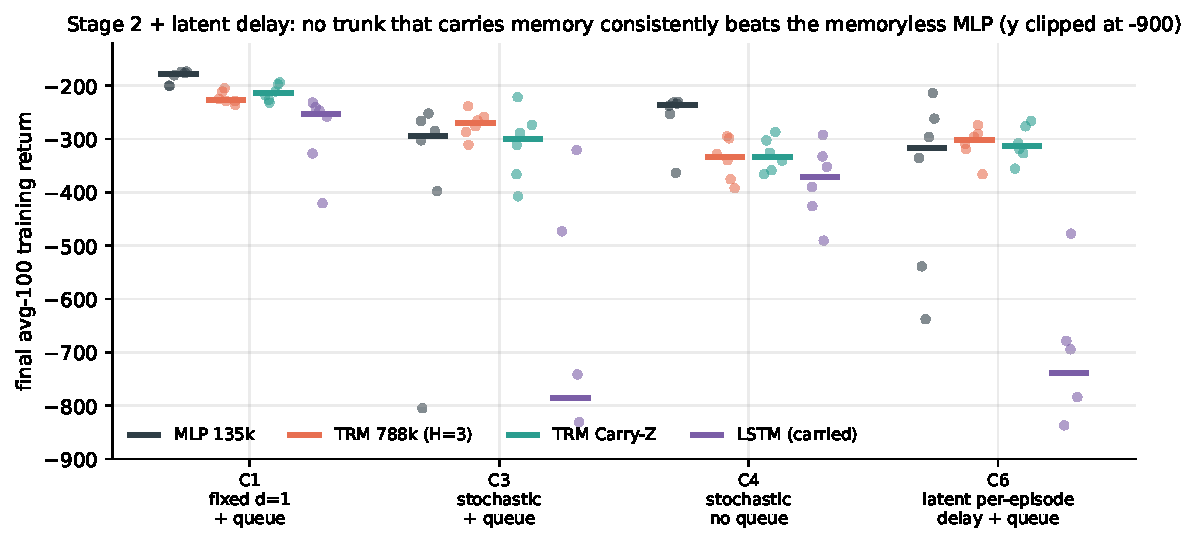
\includegraphics[width=\linewidth,height=0.42\textheight,keepaspectratio]{figures/f5_stage2.pdf}
\caption{Stage 2: uncertainty $\times$ memory}
\end{figure}



\subsection*{9.6 Supplementary --- Latent per-episode delay (G2s)}\addcontentsline{toc}{subsection}{9.6 Supplementary --- Latent per-episode delay (G2s)}



\textbf{Why this test, and its rule.} The Sep-17 plan review's central recommendation (\S{}6.3) was a delay that memory can \emph{identify}: d \textasciitilde{} U\{0..4\} drawn once at the start of each episode and held constant, with the 4-slot queue shown. A memoryless policy sees every candidate action but cannot know which slot reaches the plant. A policy that carries state could work it out from a few transitions, which is system identification. The rule, G2s, was fixed in \texttt{gates.json} before any job was submitted (Appendix A). Every trunk also sees its previous action, as in Stage 2. Five arms $\times$ 6 seeds = 30 runs.



\begin{center}\begin{tabular}{lrr}
\toprule
Arm (C6, latent per-episode delay) & Median return & Seed SD \\
\midrule
MLP 135k & $-$315.9 & 168.8 \\
MLP + oracle (the episode's delay shown) & $-$278.1 & --- \\
TRM Reset-Z & $-$302.5 & 32.0 \\
TRM Carry-Z & $-$313.2 & 33.2 \\
LSTM (carried) & $-$739.3 & --- \\
\bottomrule
\end{tabular}\end{center}



\begin{center}\small\begin{tabular}{>{\raggedright\arraybackslash}p{0.367\linewidth}>{\raggedleft\arraybackslash}p{0.184\linewidth}>{\raggedleft\arraybackslash}p{0.092\linewidth}>{\raggedright\arraybackslash}p{0.235\linewidth}}
\toprule
Contrast (n = 6) & Median & Positive & Verdict \\
\midrule
Headroom: MLP + oracle $-$ MLP & +25.2 (mean +86.4) & 4/6 & \textbf{fails} (pooled SD 128.3) \\
Carry-Z $-$ MLP & +6.3 & 3/6 & fails \\
Carry-Z $-$ Reset-Z & $-$4.9 & 2/6 & fails \\
Carried LSTM $-$ MLP & $-$432.7 & 0/6 & --- \\
Interaction [Carry-Z $-$ MLP], C6 $-$ C1 & +15.1 & 5/6 & see below \\
Interaction [Reset-Z $-$ MLP], C6 $-$ C1 & +53.0 & 4/6 & see below \\
\bottomrule
\end{tabular}\end{center}



\textbf{G2s: the H3 rejection stands.} The latent delay is expensive for every trunk: it costs the MLP 116 reward units against C1 (median per seed). But even revealing the delay does not consistently recover that cost (4/6, inside the seed spread). Carrying the latent adds nothing over resetting it (2/6), and the carried LSTM collapses.



\textbf{The one pattern that could be misread.} [Carry-Z $-$ MLP] improves from C1 to C6 in 5/6 seeds, the shape H3 predicted. It is not a memory effect.

\begin{itemize}
\item \textbf{Reset-Z, which carries nothing, shows it more strongly} (+53.0, 4/6).
\item \textbf{Its source is the MLP.} Under the latent delay the MLP collapses in two seeds (C6 $-$ C1: $-$365 and $-$458), while both TRM variants degrade uniformly ($-$60 to $-$137). Seed SD at C6 is 169 for the MLP against 32--33 for either TRM.
\end{itemize}



The real observation is that \textbf{the recursive trunks train more consistently than the MLP under a latent delay}: the MLP either copes or collapses. That concerns training stability, not inference, and it is exploratory.



\textbf{Deterministic evaluation, secondary.} On the last five evaluation episodes, Carry-Z's greedy policy beats Reset-Z's in 5/6 seeds (median +26.5). That is the only place in the study where carrying the latent shows a consistent sign, on a secondary metric at n = 6 (one-sided p = 0.109). The full battery does not confirm it. On 20 unseen-seed episodes per checkpoint, Carry-Z $-$ Reset-Z is +0.4 (4/6, p = 0.34), so the exploratory signal was noise. Deterministically, the oracle helps the MLP modestly (+12.5, 5/6). Both TRM variants' greedy policies sit slightly above the MLP's (Reset-Z +11.4, Carry-Z +15.9, 4/6 each), which again tracks the MLP's two unstable seeds rather than any use of memory.



\begin{figure}[htbp]\centering
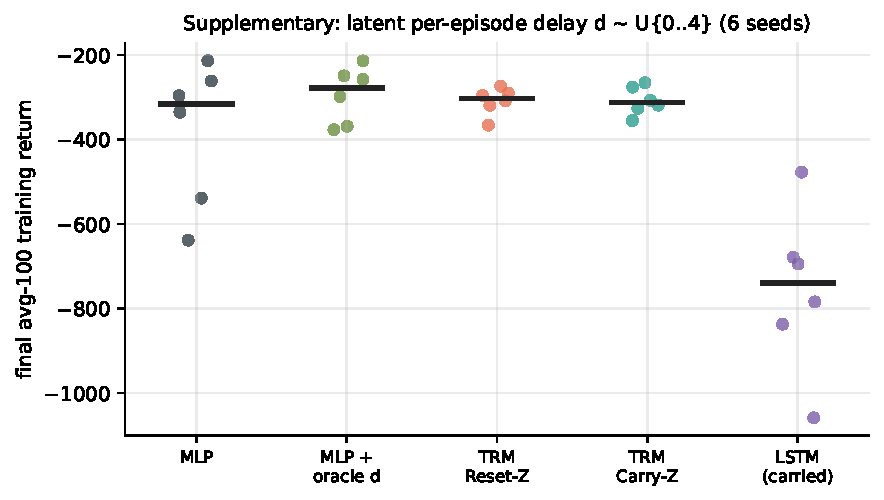
\includegraphics[width=\linewidth,height=0.42\textheight,keepaspectratio]{figures/f11_latent_delay.pdf}
\caption{Supplementary latent-delay test}
\end{figure}



\subsection*{9.7 Deployment scorecard over all Phase 3 checkpoints}\addcontentsline{toc}{subsection}{9.7 Deployment scorecard over all Phase 3 checkpoints}



All 198 Phase 3 checkpoints were run through the same battery (0 parameter-rebuild mismatches). Stage 1 now gives n = 6 seeds per cell and 12 pairs per contrast on learned policies, which the banked checkpoints (n = 3) could not.



\textbf{Stage 1 checkpoints, trained at fixed d = 1 + queue} (medians over 6 seeds):



\begin{center}\small\begin{tabular}{>{\raggedright\arraybackslash}p{0.071\linewidth}>{\raggedleft\arraybackslash}p{0.180\linewidth}>{\raggedleft\arraybackslash}p{0.103\linewidth}>{\raggedleft\arraybackslash}p{0.057\linewidth}>{\raggedleft\arraybackslash}p{0.110\linewidth}>{\raggedleft\arraybackslash}p{0.071\linewidth}>{\raggedleft\arraybackslash}p{0.087\linewidth}>{\raggedleft\arraybackslash}p{0.087\linewidth}}
\toprule
Trunk & Nominal IQM [95\% CI] & Reversals / s & abs($\Delta$u) & Noise $\sigma$ = 0.05 & Mass $\times$1.3 & Dropout 10\% & Delay d = 3 \\
\midrule
MLP 135k & $-$120.1 [$-$121.6, $-$104.0] & 9.06 & 0.805 & $-$209.3 & $-$183.6 & $-$144.8 & $-$296.4 \\
MLP 788k & $-$121.1 [$-$123.3, $-$104.9] & 2.76 & 0.398 & $-$204.0 & $-$182.9 & $-$145.1 & $-$479.2 \\
TRM 136k & $-$141.1 [$-$545.2, $-$113.6] & 2.52 & 0.488 & $-$397.8 & $-$248.5 & $-$253.0 & $-$547.4 \\
TRM 788k & $-$124.2 [$-$129.7, $-$106.7] & 0.38 & 0.227 & $-$286.7 & $-$232.7 & $-$165.3 & $-$332.2 \\
TRM H = 1 & $-$123.3 [$-$128.4, $-$105.6] & 5.09 & 1.149 & $-$349.9 & $-$238.5 & $-$190.0 & $-$303.7 \\
TRM H = 6 & $-$127.0 [$-$135.2, $-$109.6] & 0.37 & 0.076 & $-$434.5 & $-$505.9 & $-$304.0 & $-$746.9 \\
\bottomrule
\end{tabular}\end{center}



\textbf{Paired over 12 (seed, condition) pairs:}



\begin{center}\small\begin{tabular}{>{\raggedright\arraybackslash}p{0.147\linewidth}>{\raggedleft\arraybackslash}p{0.170\linewidth}>{\raggedleft\arraybackslash}p{0.170\linewidth}>{\raggedleft\arraybackslash}p{0.170\linewidth}>{\raggedleft\arraybackslash}p{0.193\linewidth}}
\toprule
Contrast & Nominal IQM & Reversals / s & abs($\Delta$u) & Drop under noise $\sigma$ = 0.05 \\
\midrule
TRM 788k $-$ MLP 135k & $-$3.6 (2/12, p = 0.039) & $-$6.0 (1/12, p = 0.006) & $-$0.6 (3/12) & $-$75.8 (2/12, p = 0.039) \\
TRM 788k $-$ MLP 788k & $-$3.9 (3/12) & $-$2.4 (1/12, p = 0.006) & $-$0.3 (3/12) & $-$66.2 (4/12) \\
TRM 136k $-$ MLP 135k & $-$3.6 (4/12) & $-$4.0 (2/12, p = 0.039) & $-$0.4 (2/12, p = 0.039) & $-$46.7 (3/12) \\
TRM H = 1 $-$ H = 3 & +0.9 (6/12) & +0.1 (6/12) & 0.0 (6/12) & $-$55.9 (5/12) \\
MLP 788k $-$ MLP 135k & $-$0.4 (5/12) & $-$0.3 (6/12) & $-$0.3 (4/12) & $-$13.1 (5/12) \\
\bottomrule
\end{tabular}\end{center}



Four findings, two of which revise the banked-checkpoint reading of \S{}9.2:



\begin{enumerate}
\item \textbf{Final policy quality is nearly matched, with a small consistent TRM deficit.} TRM's greedy policy trails the small MLP by 3.6 reward units (2/12 pairs, p = 0.039), about 0.3\% of the performance span. The training-return gap of \S{}9.4 is ten times larger.
\item \textbf{TRM commands markedly smoother torque (revising \S{}9.2).} It reverses direction about 0.4 times per second, against 9 for the small MLP and 2.8 for the matched one: fewer reversals in 11/12 pairs against each (p = 0.006). This is the plan's H3.4, \emph{regularity at matched return}, and at n = 12 it holds. The banked n = 3 checkpoints hid it because one TRM seed chattered. It is not a depth effect: H = 1 and H = 3 are indistinguishable (6/12), so it comes from the recursive cell, not from iteration.
\item \textbf{TRM is less robust across every perturbation (H3.5 is contradicted).} Under sensor noise it loses 76 more reward units than the MLP (2/12 favourable, p = 0.039). Under a 30\% heavier pendulum it drops to $-$233 against the MLP's $-$184, and under 10\% actuator dropout to $-$165 against $-$145. The deeper the recursion, the less robust (H = 6: $-$506 under the heavier plant, $-$304 under dropout). The MLP's envelope is nearly flat across all three.
\item \textbf{Delay mismatch is shared.} Every trunk trained at d = 1 holds to d = 2 and collapses at d = 3, and the pairwise contrasts in that drop are sign-inconsistent (6/12).
\end{enumerate}



\textbf{Stage 2 checkpoints} (n = 6 per contrast). Deterministically, Carry-Z's greedy policy edges out Reset-Z's at C1 (+3.6, 5/6) and is smoother than the MLP there (6/6). At C4, the MLP's greedy policy beats Carry-Z's in 6/6 seeds ($-$4.7), and the carried LSTM trails the MLP everywhere. Nothing in the deterministic evaluation reverses the G2 or G3 conclusions.



\textbf{What the scorecard says as a whole.} TRM is a real trade, not a dominated point. It buys much smoother actuation at a small cost in final return. It pays for that with 65$\times$ decision latency, 11--13$\times$ training cost, and a narrower robustness envelope. For a plant where actuator wear dominates and the environment is benign, the trade could be worth making. For the delay-robustness brief of this project, it is not.



\begin{figure}[htbp]\centering
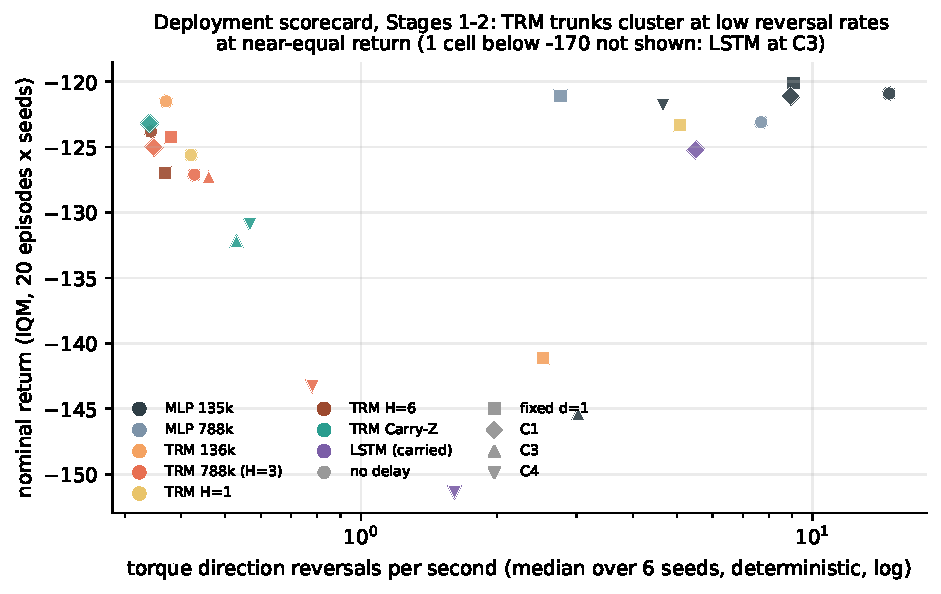
\includegraphics[width=\linewidth,height=0.42\textheight,keepaspectratio]{figures/f8_scorecard.pdf}
\caption{Deployment scorecard: return vs torque direction reversals over Stage 1--2 checkpoints}
\end{figure}



\begin{figure}[htbp]\centering
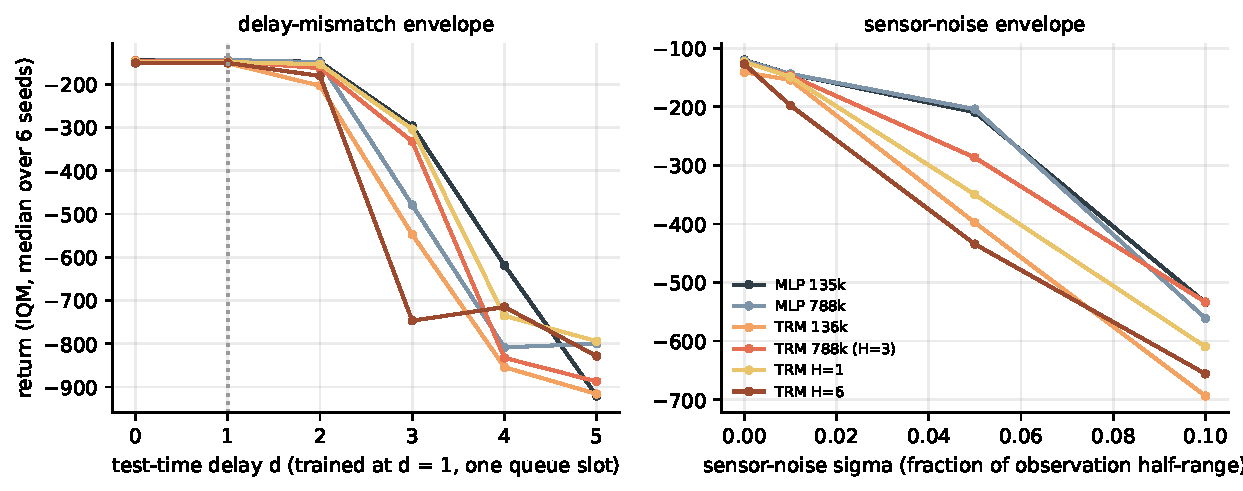
\includegraphics[width=\linewidth,height=0.42\textheight,keepaspectratio]{figures/f9_robustness.pdf}
\caption{Robustness envelopes, Stage 1 checkpoints trained at fixed d = 1}
\end{figure}



\subsection*{9.8 The cost ledger, three ways}\addcontentsline{toc}{subsection}{9.8 The cost ledger, three ways}



\begin{center}\small\begin{tabular}{>{\raggedright\arraybackslash}p{0.401\linewidth}>{\raggedright\arraybackslash}p{0.533\linewidth}}
\toprule
Reading & TRM 788k vs MLP 135k (Pendulum-v1) \\
\midrule
\textbf{Matched episodes} (the pre-registered comparison) & $-$34.4 training return (0/12); about $-$2.5 on deterministic evaluation \\
\textbf{Matched wall-clock} (when the MLP finishes, about 3 min) & TRM has completed 16 episodes; avg-10 return $-$967 against the MLP's final $-$174 \\
\textbf{Matched inference latency} & 65$\times$ slower per decision on one CPU thread (4.13 vs 0.064 ms p99) \\
Training cost, same GPU model & 10.8$\times$ (A100), 11.7$\times$ (L40S), 13.0$\times$ (V100) \\
\bottomrule
\end{tabular}\end{center}



The shallow TRM (H = 1) halves the training premium (6--8$\times$) and has the best matched-wall-clock reading of the TRM family (avg-10 $-$251 after 42 episodes). It still loses on every reading, but it is the variant to use if a recursive trunk is required.



\begin{figure}[htbp]\centering
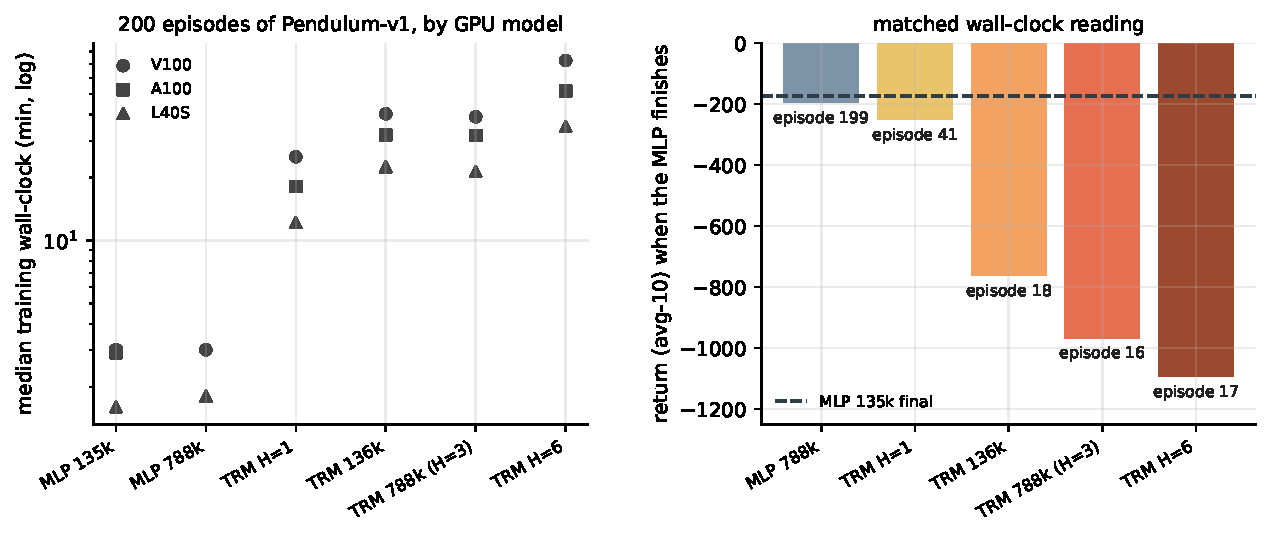
\includegraphics[width=\linewidth,height=0.42\textheight,keepaspectratio]{figures/f7_cost.pdf}
\caption{Cost ledger}
\end{figure}



\medskip



\section*{10. Synthesis across phases}\addcontentsline{toc}{section}{10. Synthesis across phases}



\begin{center}\small\begin{tabular}{>{\raggedright\arraybackslash}p{0.247\linewidth}>{\raggedright\arraybackslash}p{0.439\linewidth}>{\raggedright\arraybackslash}p{0.220\linewidth}}
\toprule
Claim & Evidence & Strength \\
\midrule
On Pendulum-v1, TRM trails the MLP on training return & Phase 1 0/6; Stage 1 0/12 ($-$34.4) & replicated, p = 0.0005 \\
The deficit is not a capacity artefact & matched-capacity losses at 135k (0/12) and 788k (2/12); MLP capacity inert (5/12) & strong \\
The final greedy policies are close to equivalent & deterministic eval within \textasciitilde{}5 units; battery TRM $-$ MLP $-$3.6 (2/12, p = 0.039), about 0.3\% of span & small but consistent TRM deficit \\
TRM fits its value function worse, architecturally & critic loss 1.45$\times$ / 1.89$\times$ at matched capacity, 12/12 each; bigger MLP fits better & strong \\
Recursion depth adds cost, not return & H $\in$ \{1, 3, 6\} flat (5/12, 4/12); latency and training cost scale with H & strong \\
Carrying the latent does not help & G3: never $\geq$ 5/6 at any condition (C1, C3, C4; C6 2/6) & moderate: n = 6 excludes only consistent effects \\
Memory does not recover delay headroom & G2 wrong sign at C4 (1/6); carried LSTM worse everywhere; latent-delay test fails its rule & moderate \\
TRM commands smoother torque at matched return (H3.4) & 0.4 vs 9 reversals/s, 11/12 pairs, p = 0.006 & supported at n = 12 \\
TRM degrades more gracefully off-nominal (H3.5) & worse under noise (2/12), heavier plant and dropout; deeper is worse & contradicted \\
TRM is a worse controller to deploy & 65$\times$ latency, 11--13$\times$ training cost, narrower robustness envelope & strong on cost and robustness \\
Complexity scaling (the original H1) & two of three rungs were floor effects & \textbf{untested}, not disconfirmed \\
The recursive structure (base, hier6, singlez) matters & sign-inconsistent on a floor-effect environment & not established either way \\
\bottomrule
\end{tabular}\end{center}



\textbf{What the three confounds became.}

\begin{itemize}
\item \textbf{C-1 (capacity):} removed by the Stage 1 2$\times$2. The result is architectural.
\item \textbf{C-2 (latent reset):} removed by Carry-Z with exact stored-state replay. The result is unchanged.
\item \textbf{C-3 (nothing to infer):} removed by showing real memory headroom (G0), and probed again with a latent delay built to be identifiable from history (G2s), where even an oracle gained only inconsistently. No trunk exploited either.
\end{itemize}



The Phase 1--2 negative was therefore not an artefact of any of the three.



\textbf{What the result is about.} TRM's in-domain success depends on a supervised training discipline this port lacks: deep supervision across a refinement trajectory against a fixed answer, per-instance embeddings, and test-time compute (ARC Prize, 2025; Roye-Azar et al., 2026). With that discipline absent, the recursive computation behaves like an expensive, harder-to-optimise feed-forward block whose extra depth goes unused (7 of 21 applications trained, depth inert). Stage 4 would have tested restoring it; its gate (G3) did not open, and the plan is explicit that running it now would be exploratory rather than confirmatory.



\medskip



\section*{11. Threats to validity}\addcontentsline{toc}{section}{11. Threats to validity}



\begin{itemize}
\item \textbf{One validated environment.} Every decisive Phase 3 test ran on Pendulum-v1. Stage 3's unstable plant (InvertedDoublePendulum-v5) was gated on G2 and not run.
\item \textbf{One learning algorithm.} DDPG throughout. The TD3 cross-check was gated on G2; TD3 support for Carry-Z is built but unused.
\item \textbf{Seeds.} 6 per cell, with gates at $\geq$ 5/6 (one-sided p = 0.109). The design detects consistent effects, not small ones. Two-sided p-values are reported alongside.
\item \textbf{The primary metric includes exploration noise.} Training avg-100 was pre-registered for continuity with Phases 1--2. \S{}9.4 shows the deterministic reading is much closer, and conclusions about \emph{final policy quality} rest on the battery, not on the gates.
\item \textbf{A-6 changed the Stage 2 baseline.} The previous-action input closed most of C4's headroom for the MLP. The failure survives the stricter comparison against a history-free MLP, but that comparison crosses two stages rather than being built into one design.
\item \textbf{The carried LSTM was not tuned.} It is a weak memory baseline, as the Phase 1 LSTM was. Carry-Z beating it is not evidence for recursion.
\item \textbf{Stored-state replay only.} The burn-in variant the plan kept in reserve was not needed: Carry-Z was not close to passing, it was indistinguishable from Reset-Z.
\item \textbf{Hardware.} GPU models varied. Costs are compared within a model, and latency on one fixed machine.
\item \textbf{Plan-review timing.} The Sep-17 review was not consulted before execution. Its central fix was run afterwards as a supplementary test with its rule fixed before data, and its other recommendations are accounted for in \S{}6.3.
\item \textbf{Gate operationalisation.} G4's rule did not exclude untrained policies. It is reported as written, with the degenerate pass named. G4 was evaluated on the banked n = 3 checkpoints as pre-registered. The n = 12 Stage 1 scorecard supports TRM's non-dominance on smoothness more strongly than G4's own evidence did.
\end{itemize}



\medskip



\section*{12. Recommendations and open questions}\addcontentsline{toc}{section}{12. Recommendations and open questions}



\textbf{For practice.} Use the MLP for delay-conditioned model-free control at this scale. Where a recursive trunk is wanted anyway, use \texttt{H\_cycles = 1}: it matches deeper variants on return at a third of the latency.



\textbf{For science, in order of value:}

\begin{enumerate}
\item \textbf{Restore the training discipline (plan Stage 4):} backpropagate through all cycles, and supervise every outer cycle's readout. This is the one remaining route to a constructive positive result, and the literature points at it. It should be run as exploration, since G3 did not open it.
\item \textbf{Generalise the negative:} the decisive contrast under TD3, and on an environment that is learned at budget and open-loop unstable (InvertedDoublePendulum-v5 after a budget pilot). Everything needed is built.
\item \textbf{Re-test complexity scaling properly:} the original H1 remains untested, because two of its three rungs were floor effects. Any new rung needs a budget pilot first.
\item \textbf{A tuned recurrent baseline} (Ni et al., 2022) before any claim about memory in this setting.
\end{enumerate}



\medskip



\section*{13. Reproducibility}\addcontentsline{toc}{section}{13. Reproducibility}



\begin{itemize}
\item \textbf{Code.} Training entry point \texttt{main.py} (Hydra). New Phase 3 code: \texttt{src/delays.py}, \texttt{src/\allowbreak{}perturb.\allowbreak{}py}, \texttt{src/eval.py}, \texttt{src/\allowbreak{}models/\allowbreak{}trm\_\allowbreak{}control.\allowbreak{}py::TRMCarryTrunk}, \texttt{src/\allowbreak{}models/\allowbreak{}lstm\_\allowbreak{}control.\allowbreak{}py::LSTMCarryTrunk}, \texttt{src/\allowbreak{}algos/\allowbreak{}\{ddpg,\allowbreak{}td3\}.\allowbreak{}py}. New configs: \texttt{conf/\allowbreak{}model/\allowbreak{}\{trm\_\allowbreak{}small,\allowbreak{}trm\_\allowbreak{}h1,\allowbreak{}trm\_\allowbreak{}h6,\allowbreak{}trm\_\allowbreak{}carryz,\allowbreak{}lstm\_\allowbreak{}carry,\allowbreak{}dnn\_\allowbreak{}large\}.\allowbreak{}yaml}, \texttt{conf/\allowbreak{}delay/\allowbreak{}\{stochastic\_\allowbreak{}u4,\allowbreak{}episode\_\allowbreak{}u4\}.\allowbreak{}yaml}, \texttt{conf/\allowbreak{}env/\allowbreak{}invdoublependulum.\allowbreak{}yaml}.
\item \textbf{Job tooling.} \texttt{experiments/\allowbreak{}phase3/\allowbreak{}p3.\allowbreak{}py} (manifests, submission, status), \texttt{sync.sh} (frozen per-stage snapshots on Katana), \texttt{w0\_eval.py}, \texttt{bench\_\allowbreak{}latency.\allowbreak{}py}.
\item \textbf{Analysis.} \texttt{experiments/\allowbreak{}phase3/\allowbreak{}gates\_\allowbreak{}eval.\allowbreak{}py} (gate rules), \texttt{extract\_\allowbreak{}runs.\allowbreak{}py}, \texttt{analyze\_\allowbreak{}phase3.\allowbreak{}py}, \texttt{make\_\allowbreak{}figures\_\allowbreak{}phase3.\allowbreak{}py}. Outputs: \texttt{experiments/\allowbreak{}analysis\_\allowbreak{}p3\_\allowbreak{}g0.\allowbreak{}json}, \texttt{analysis\_\allowbreak{}w0.\allowbreak{}json}, \texttt{analysis\_\allowbreak{}s1.\allowbreak{}json}, \texttt{analysis\_\allowbreak{}s2.\allowbreak{}json}, \texttt{analysis\_\allowbreak{}phase3\_\allowbreak{}full.\allowbreak{}json}.
\item \textbf{Data.} Raw results in \texttt{results\_\allowbreak{}phase3/\allowbreak{}} locally and under \texttt{/\allowbreak{}srv/\allowbreak{}scratch/\allowbreak{}z5308482/\allowbreak{}trm-control/\allowbreak{}} on Katana. Checkpoints in \texttt{models/}, named by each run's \texttt{model\_id}. The job ledger is \texttt{\textasciitilde{}/\allowbreak{}jobs/\allowbreak{}phase3/\allowbreak{}ledger.\allowbreak{}jsonl}.
\item \textbf{One training run}, e.g. Stage 2 Carry-Z at C4, seed 1:
\end{itemize}



{\small\begin{verbatim}
python3 main.py arch=ddpg model=trm_carryz env=pendulum \
  delay=stochastic_u4 augment_obs=false prev_action_obs=true \
  run_tag=pa arch.total_episodes=200 seed=1 wandb.enabled=false
\end{verbatim}}



\medskip



\section*{Appendix A --- Gate rules as fixed before their data}\addcontentsline{toc}{section}{Appendix A --- Gate rules as fixed before their data}



\begin{center}\small\begin{tabular}{>{\raggedright\arraybackslash}p{0.063\linewidth}>{\raggedright\arraybackslash}p{0.580\linewidth}>{\raggedright\arraybackslash}p{0.263\linewidth}}
\toprule
Gate & Rule & Outcome \\
\midrule
G0 & Per seed, final return. Passes if oracle headroom (A3 $-$ A2) \emph{or} memory headroom (A2 $-$ A4) has median above the pooled seed SD and is positive in $\geq$ 5/6 seeds. & pass (memory headroom only) \\
G1 & n = 12 (seed, condition) pairs. "Different" = $\geq$ 10/12 share a sign. Stage 2 MLP = \texttt{dnn\_large} iff MLP capacity is different, else \texttt{dnn}. & decided; \texttt{dnn} \\
G2 & [Carry-Z $-$ MLP] relative to C1, at C3 or C4 (co-primary), positive in $\geq$ 5/6 seeds. & fail \\
G3 & Carry-Z beats Reset-Z in $\geq$ 5/6 seeds at some condition. & fail \\
G4 & Pendulum fixed-delay checkpoints: a non-MLP trunk non-dominated against the MLP on (return, command rate) and admitting 100 Hz at CPU p99. & weak pass (literal) \\
G2s & Latent per-episode delay. Headroom (oracle $-$ MLP) passes as G0 does; H3 survives, narrowed, only if Carry-Z also beats both the MLP and Reset-Z in $\geq$ 5/6 seeds. & rejection stands (headroom 4/6; Carry-Z $-$ Reset-Z 2/6) \\
\bottomrule
\end{tabular}\end{center}



\section*{Appendix B --- Where Phase 3 departed from the plan}\addcontentsline{toc}{section}{Appendix B --- Where Phase 3 departed from the plan}



\begin{itemize}
\item \textbf{Stage 0 on GPU, not CPU} (author direction). The battery ran as shard jobs rather than one job per checkpoint.
\item \textbf{Stage 1 ran alongside Stage 0}, not after it. It is not gated by G0.
\item \textbf{Arm A4, the C4 co-primary and the previous-action input} were added before any data (A-2, A-3, A-6).
\item \textbf{The latent-delay test} was added after G2, with its rule fixed before its data.
\item \textbf{The battery was run over all 198 Phase 3 checkpoints} for the synthesis. It was not in the plan, which covered only the banked checkpoints.
\item \textbf{Stages 3 and 4 were not run}, per G2 and G3.
\end{itemize}



\section*{References}\addcontentsline{toc}{section}{References}



Agarwal, R. et al. (2021). \emph{Deep Reinforcement Learning at the Edge of the Statistical Precipice.} NeurIPS. arXiv:2108.13264 $\cdot$ ARC Prize (2025). \emph{The Hidden Drivers of HRM's Performance on ARC-AGI.} $\cdot$ Bai, S., Kolter, J. Z. \& Koltun, V. (2019). \emph{Deep Equilibrium Models.} NeurIPS. $\cdot$ Dang, L. H. \& Rawlinson, D. (2025). \emph{HRM-Agent.} arXiv:2510.22832 $\cdot$ Derman, E., Dalal, G. \& Mannor, S. (2021). \emph{Acting in Delayed Environments with Non-Stationary Markov Policies.} ICLR. $\cdot$ Jain, A. \& Linares, R. (2025). \emph{Tiny Recursive Control.} arXiv:2512.16824 $\cdot$ Jolicoeur-Martineau, A. (2025). \emph{Less is More: Recursive Reasoning with Tiny Networks.} arXiv:2510.04871 $\cdot$ Katsikopoulos, K. V. \& Engelbrecht, S. E. (2003). Markov decision processes with delays and asynchronous cost collection. \emph{IEEE TAC} 48(4) $\cdot$ Kapturowski, S. et al. (2019). \emph{Recurrent Experience Replay in Distributed RL (R2D2).} ICLR $\cdot$ Klein, T. et al. (2024). \emph{Plasticity Loss in Deep RL: A Survey.} arXiv:2411.04832 $\cdot$ Lee, C.-Y. et al. (2015). \emph{Deeply-Supervised Nets.} AISTATS $\cdot$ Lillicrap, T. P. et al. (2016). \emph{Continuous control with deep reinforcement learning.} ICLR $\cdot$ Matheron, G., Perrin, N. \& Sigaud, O. (2019). \emph{The problem with DDPG.} arXiv:1911.11679 $\cdot$ Ni, T., Eysenbach, B. \& Salakhutdinov, R. (2022). \emph{Recurrent Model-Free RL Can Be a Strong Baseline for Many POMDPs.} ICML $\cdot$ Ota, K., Jha, D. K. \& Kanezaki, A. (2021). \emph{Training Larger Networks for Deep RL.} arXiv:2102.07920 $\cdot$ Roye-Azar, A. et al. (2026). \emph{Tiny Recursive Models on ARC-AGI-1.} arXiv:2512.11847 $\cdot$ Wijayatunga, M. \& Armellin, R. (2026). \emph{Tiny Recursive Models for Solving the J2-Perturbed Lambert Problem.} arXiv:2606.00895
\end{document}
